\section{Slicing triangulated categories} 
\epigraph{\textit{I do not understand the definition of a Gorenstein ring.}}{Daniel Gorenstein}
\vspace{10 mm}

We now come to the main topic of this thesis. Using \hyperref[p]{\textbf{Proposition \ref*{p}}} as a guide, we give the notion of 'slicing' on a triangulated category, generalizing bounded t-structures. These first appeared in \cite{bri} as a way to formalize string-theoretic ideas of stability. Our approach is slightly more general and goes along the lines of \cite{gor}. But first, we need some combinatorial tools. \\

\begin{defn}
A $\mathbb{Z}$-\textbf{poset} is a poset $J$ equipped with a group action by $\mathbb{Z}$ so that the action map $$\mathbb{Z} \times J \longrightarrow J$$ is a a morphism of posets (i.e. non decreasing), where the left member has the product order. 
\end{defn} 

We write the action as $\phi+i$, with $\phi \in J$ and $i \in \mathbb{Z}$. The $\mathbb{Z}$-posets clearly define a category, denoted $\textnormal{Pos}_{\mathbb{Z}}$, where the morphisms are $\mathbb{Z}$-equivariant morphisms of posets. Just like the category of posets, this is a cartesian closed category. We further denote $\textnormal{tPos}_{\mathbb{Z}}$ the full subcategory of totally ordered $\mathbb{Z}$-posets. \\

\begin{exmp}
The poset $\mathfrak{ts}(\mathscr{D})$ is a $\mathbb{Z}$-poset with $\mathbb{Z}$ acting by translation, and $\mathfrak{bts}(\mathscr{D}) \subseteq \mathfrak{ts}(\mathscr{D})$ is a sub-$\mathbb{Z}$-poset. While we will almost always assume our $\mathbb{Z}$-posets to be totally ordered, this is the main reason why we don't put it into the definition. 
\end{exmp}

Let $J$ be a $\mathbb{Z}$-poset. From now on, \textit{we will asume that our posets and $\mathbb{Z}$-posets are totally ordered}. \\
%\begin{defn}
%We call \textbf{Alexandrov presheaf of t-structures} a morphism of $\mathbb{Z}$-posets $O(J)^{\textnormal{op}} \overset{\mathscr{F}}{\longrightarrow} \textnormal{ts}(\mathscr{D})^{\textnormal{op}}$. We denote $$\textnormal{Apt}_J(\mathscr{D}) = \textnormal{Hom}_{\textnormal{Pos}_{\mathbb{Z}}}(O(J)^{\textnormal{op}},\textnormal{ts}(\mathscr{D})^{\textnormal{op}})$$ and for $\phi \in J$
%\begin{align*} 
%\tau^{\ge \phi}_{\mathscr{F}}&=\tau^{\ge}_{\mathscr{F}([\phi, + \infty[)} &  \tau^{< \phi}_{\mathscr{F}}&=\tau^{<}_{\mathscr{F}([\phi, + \infty[)} \\  \tau^{> \phi}_{\mathscr{F}}&=\tau^{\ge}_{\mathscr{F}(]\phi, + \infty[)} &  \tau^{\le \phi}_{\mathscr{F}}&=\tau^{<}_{\mathscr{F}(]\phi, + \infty[)}
%\end{align*}  
% $$H^{\phi}_{\mathscr{F}}=\tau^{\ge \phi}_{\mathscr{F}}\tau^{\le \phi}_{\mathscr{F}}=\tau^{\le \phi}_{\mathscr{F}}\tau^{\ge \phi}_{\mathscr{F}}$$
%We call \textbf{support} of $X \in \mathscr{D}$ with respect to $\mathscr{F}$ the set 
%We say that $X \in \mathscr{D}$ is \textbf{semistable of phase} $\phi$ with respect to $\mathscr{F}$ if $H^{\phi}_{\mathscr{F}}(X)=X$, we denote $\mathscr{P}^{\mathscr{F}}_{\phi}$ the full subcategory of semistables of phase $\phi$ and for each subset $I \subseteq J$ we set $$\mathscr{P}^{\mathscr{F}}_I = \left\langle \bigcup_{\phi \in I } \mathscr{P}^{\mathscr{F}}_{\phi} \right\rangle$$  We say that $X$ is of \textbf{finite support} if $\textnormal{supp}_{\mathscr{F}}(X)$ is finite, and in this case and if $J$ is totally ordered denote $$\phi^+_{\mathscr{F}}(X)=\max \textnormal{supp}_{\mathscr{F}}(X)$$ $$\phi^-_{\mathscr{F}}(X)=\min \textnormal{supp}_{\mathscr{F}}(X)$$ 
%We say that $\mathscr{F}$ is of finite support if each $X \in \mathscr{D}$ is. 
%\end{defn}
%
%Composing the functor $\textnormal{Hom}_{\textnormal{Pos}_{\mathbb{Z}}}(*,\textnormal{ts}(\mathscr{D})^{\textnormal{op}})$ with the functor $O(*)^{\textnormal{op}}$ we obain that the Aleaxandrov presheaves of t-structures define a functor $$\textnormal{Pos}_{\mathbb{Z}} \xrightarrow{\textnormal{Apt}_*(\mathscr{D})} \textnormal{Pos}_{\mathbb{Z}}$$
%We denote by $*^!$ the value of that functor on morphisms. Observe that Proposition ??? gives us a natural transformation $$\textnormal{Apt}_*(\mathscr{D}) \longrightarrow \mathscr{D}^{\mathscr{D} \times O(*)^{\textnormal{op}}}$$
%Moreover, $\textnormal{Aut}(\mathscr{D})$ still acts on $\textnormal{Apt}(\mathscr{D})$ pointwise; in other words we set $(F.\mathscr{F})(I)=F(\mathscr{F}(I))$ for each $I \in O(J)$.  Clearly, we again have $$H^{\phi}_{F.\mathscr{F}}=F H^{\phi}_{\mathscr{F}} F^{-1}$$
%Now, let $\mathscr{F} \in \textnormal{Apt}_J(\mathscr{D})$ be an Alexandrov sheaf of t-structures. 
%
%\begin{prop}
%Let $J \overset{f}{\longrightarrow} J'$ be a morphism of totally ordered $\mathbb{Z}$-posets. For each $\phi \in J$ $$H^{\phi}_{\mathscr{F}}=H^{\phi}_{\mathscr{F}}H^{f(\phi)}_{f^!(\mathscr{F})}$$
%\end{prop}
%
%\begin{proof}
%Since we have inclusions $$f^{-1}(] f(\phi), + \infty [) \subseteq ]\phi, +\infty[ \subseteq [\phi, +\infty[ \subseteq f^{-1}([ f(\phi), + \infty [)$$
%\hyperref[l]{\textbf{Proposition \ref*{l}}} gives us 
%\begin{align*} 
%H^{\phi}_{\mathscr{F}}&= \tau^{\le \phi}_{\mathscr{F}} \tau^{\ge \phi}_{\mathscr{F}} \\ &= \tau^{\le \phi}_{\mathscr{F}} \tau^{\le f(\phi)}_{f^!(\mathscr{F})}\tau^{\ge f(\phi)}_{f^!(\mathscr{F})}\tau^{\ge \phi}_{\mathscr{F}} \\ &= \tau^{\le \phi}_{\mathscr{F}} \tau^{\ge \phi}_{\mathscr{F}} \tau^{\le f(\phi)}_{f^!(\mathscr{F})}\tau^{\ge f(\phi)}_{f^!(\mathscr{F})}= H^{\phi}_{\mathscr{F}}H^{f(\phi)}_{f^!(\mathscr{F})} 
%\end{align*}
%as desired. 
%\end{proof}
%
%Now, observe that by Proposition ???  $H^{\phi}_{\mathscr{F}}$ is idemponent ($H^{\phi}_{\mathscr{F}}H^{\phi}_{\mathscr{F}}=H^{\phi}_{\mathscr{F}}$) for each $\phi \in J$, and thus $H^{\phi}_{\mathscr{F}}(X)$ is semistable for each $X \in \mathscr{D}$. 
%
%\begin{prop}
%If $J$ is totally ordered and $0 \not = X \in \mathscr{D}$ is semistable of phase $\phi$, then $\textnormal{supp}_{\mathscr{F}}(X)= \{ \phi \}$. 
%\end{prop}
%
%\begin{proof}
%First of all, since $H^{\phi}_{\mathscr{F}}$ is idempotent and $X \not = 0$, $\phi \in \textnormal{supp}_{\mathscr{F}}(X)$. Pick $\psi \not = \phi$. Since $J$ is totally ordered, we have $\psi < \phi$ or $\phi > \psi$. Assuming that we are in the first situation (the proof in the other case is done similarly), we have $$H^{\psi}_{\mathscr{F}}H^{\phi}_{\mathscr{F}}= \tau^{\ge \psi}_{\mathscr{F}}\tau^{\le \psi}_{\mathscr{F}}\tau^{\ge \phi}_{\mathscr{F}}\tau^{\le \phi}_{\mathscr{F}}$$
%But since $[\phi, +\infty[ \subseteq] \psi, + \infty[$, we se by the first equality of Proposition ??? that $\tau^{\le \psi}_{\mathscr{F}}\tau^{\ge \phi}_{\mathscr{F}}=0$, as desired. 
%\end{proof} 
%
%\begin{defn}
%We say that $\mathscr{F}$ is \textbf{regular} if for each $0 \not = X \in \mathscr{D}$, $X$ is semistable of phase $\phi$ whenever $\textnormal{supp}_{\mathscr{F}}(X)=\{ \phi \}$. 
%\end{defn}
%
%\begin{prop}
%Suppose that $J$ is totally ordered and that $X$ is of finite support. If we denote $$\textnormal{supp}_{\mathscr{F}}(X)= \{ \phi^+_{\mathscr{F}}(X)= \phi_1 > \cdots > \phi_n= \phi^-_{\mathscr{F}}(X) \} $$ then the cone of the natural transformation induced by $\tau_{\mathscr{F}}^{\ge *}(X)$ on $\phi_i > \phi_{i-1}$ is $H^{\phi_i}_{\mathscr{F}}(X)$ for each $i>1$ and $\tau^{\ge \phi_n}_{\mathscr{F}}(X)=X$. 
%\end{prop}
%
%\begin{proof}
%By the last claim of Proposition, the cone of the statement is $A=\tau^{< \phi_{i-1}}_{\mathscr{F}} \tau^{\ge \phi_i}_{\mathscr{F}}(X)$. Suppose that $H^{\phi_i}_{\mathscr{F}}(X) \not = A$. Since $H^{\phi_i}_{\mathscr{F}}(A)=H^{\phi_i}_{\mathscr{F}}(X)$ by idempotency, we have that $A$ is not semistable of phase $\phi_i$. But then there must be a $\phi_i < \psi < \phi_{i-1}$ so that $H^{\psi}_{\mathscr{F}}(A) \not = 0$. By another usual computation,  $H^{\psi}_{\mathscr{F}}(X)=H^{\psi}_{\mathscr{F}}(A) \not = 0$, which means that $\psi \in \textnormal{supp}_{\mathscr{F}}(X)$, which is absurd since there are not elements in the support of $X$ between $\phi_i$ and $\phi_{i-1}$. 
%\end{proof}
%
%
%\begin{prop}
%Suppose that $J$ is totally ordered. For each $I \in O(J)$, $\mathscr{F}(I)^{\perp}=\mathscr{P}^{\mathscr{F}}_{J \setminus I}$. 
%\end{prop}
%
%\begin{proof}
%  Since $X \in \mathscr{F}(I)^{\perp}$ if a and only if $\tau^{\ge}_{\mathscr{F}(I)}(X)=0$ if and only if $\tau^<_{\mathscr{F}}(X)=X$, we have that for each $\phi in I$ BOH NON LO SO, SONO STANCO
%\end{proof}
%
%In particular, we have that for each $\phi \in J$, $\mathscr{P}^{\mathscr{F}}_{ \{ \phi \}}=\mathscr{P}^{\mathscr{F}}_{\phi}$, and thus $\mathscr{P}^{\mathscr{F}}_{\phi}$ is extension-closed. \\
%
%
%\begin{prop}
%Let $J \overset{f}{\longrightarrow} J'$ be a morphism of totally ordered $\mathbb{Z}$-posets, $I \subseteq J'$ an interval. Then $$\mathscr{P}^{f^!(\mathscr{F})}_I= \mathscr{P}^{\mathscr{F}}_{f^{-1}(I)}$$
%\end{prop}
%
%\begin{proof}
%Observe that is suffices to show the statement for $I=\{ \psi \}$ a singleton. Now for each $\phi \in f^{-1}(\psi)$, if $X \in \mathscr{P}^{\mathscr{F}}_{\phi}$, since $H^{\phi}_{\mathscr{F}}(X)=X$, by Proposition ??? we get $$H^{\psi}_{f^!(\mathscr{F})}(X)=X$$ and thus $X \in \mathscr{P}^{f^!(\mathscr{F})}_{\psi}$. This shows that $\mathscr{P}^{\mathscr{F}}_{\phi} \subseteq \mathscr{P}^{f^!(\mathscr{F})}_{\psi}$ for each $\phi \in f^{-1}(\psi)$, and thus, by extension-closeness, $\mathscr{P}^{\mathscr{F}}_{f^{-1}(\psi)} \subseteq \mathscr{P}^{f^!(\mathscr{F})}_{\psi}$. \\
%Now, let $X \in \mathscr{P}^{f^!(\mathscr{F})}_{\psi}$. Suppose that $X \not \in \mathscr{P}^{\mathscr{F}}_{f^{-1}(\psi)} $. Then, by Proposition ???, there is $\phi \in \textnormal{supp}_{\mathscr{F}}(X)$ so that $f(\phi) \not = \psi$. But Proposition ??? again tells us that $$0 \not = H^{\phi}_{\mathscr{F}}(X)=  H^{\phi}_{\mathscr{F}}( H^{f(\phi)}_{f^!(\mathscr{F})}(X))$$
%and thus $H^{f(\phi}_{f^!(\mathscr{F})}(X) \not = 0$, which means that $\psi \not = f(\phi) \in \textnormal{supp}_{f^!(\mathscr{F})}(X)$, which contradicts the semistability of $X$ with respect to $f^!(\mathscr{F})$. 
%\end{proof}
%
%\begin{prop}
%Let $J \overset{f}{\longrightarrow} J'$ be a morphism of totally ordered $\mathbb{Z}$-posets, $X \in \mathscr{D}$ of finite support with respecto to $\mathscr{F}$ $$f(\textnormal{supp}_{\mathscr{F}}(X))=\textnormal{supp}_{f^!(\mathscr{F})}(X)$$ 
%In particular, $X$ is of finite support with respect to $f^!(\mathscr{F})$.
%\end{prop}

%\begin{proof}
%The inclusion $f(\textnormal{supp}_{\mathscr{F}}(X)) \subseteq \textnormal{supp}_{f^!(\mathscr{F})}(X)$ is proven with the same computation as in the second part of Proposition ???. For the other inclusion, pick $\psi \in \textnormal{supp}_{f^!(\mathscr{F})}(X)$. Since $H^{\psi}_{f^!(\mathscr{F})}(X) \in \mathscr{P}^{f^!(\mathscr{F})}_{\psi}=\mathscr{P}^{\mathscr{F}}_{f^{-1}(\psi)}$ (the last equality is given by Proposition ???), by Proposition ??? $\textnormal{supp}_{\mathscr{F}}(H^{\psi}_{f^!(\mathscr{F})}(X)) \subseteq f^{-1}(\psi)$. Picking $\phi \in \textnormal{supp}_{\mathscr{F}}(H^{\psi}_{f^!(\mathscr{F})}(X))$, we see by Proposition ??? that $$0 \not = H^{\phi}_{\mathscr{F}}(H^{\psi}_{f^!(\mathscr{F})}(X))=H^{\phi}_{\mathscr{F}}(X)$$ which means that $\phi \in \textnormal{supp}_{\mathscr{F}}(X)$, as desired. 
%\end{proof}
%
%Let $J$ be a $\mathbb{Z}$-poset. \\
%
%\begin{defn}
%A \textbf{bounded} $J$-\textbf{family} of t-structures on $\mathscr{D}$ is a morphism of $\mathbb{Z}$-posets $J \overset{\mathscr{F}}{\longrightarrow} \textnormal{ts}(\mathscr{D})^{\textnormal{op}}$ so that $$\mathscr{D}=\bigcup_{i,j \in J}(\mathscr{F}(i) \cap \mathscr{F}(j)^{\perp})$$
%\end{defn}
%
%If $\mathfrak{t}$ is a t-structure on $\mathscr{D}$, we have a morphism of $\mathbb{Z}$-posets $\mathbb{Z} \longrightarrow \textnormal{ts}(\mathscr{D})^{\textnormal{op}}$ which sends $0$ to $\mathfrak{t}$. We will say that $\mathfrak{t}$ is bounded if the latter morphism is a bounded family, and we denote $\textnormal{bts}(\mathscr{D})$ the sub-$\mathbb{Z}$-poset of $\textnormal{ts}(\mathscr{D})$ consisting of bounded t-structure of $\mathscr{D}$. If $\mathfrak{t} \in \textnormal{bts}(\mathscr{D})$, we denote $\heartsuit_{\mathfrak{t}}=\mathfrak{t}\cap \mathfrak{t}^{\perp}[1]$.\\
%The following proposition is the crucial motivation for the following definitions. 
%
%\begin{prop}
%Let $\mathfrak{t}$ be a bounded t-structure on $\mathscr{D}$. Then for each $0 \not = X \in \mathscr{D}$ there is a finite strictly decreasing sequence of integers $\{ \phi_1 > \dots > \phi_n \} \subseteq \mathbb{Z}$ and a factorization of the initial morphism $$0=X_0 \overset{\alpha_1}{\longrightarrow} \cdots \overset{\alpha_n}{\longrightarrow} X_n=X$$ so that $0 \not = \textnormal{cone}(\alpha_i) \in \heartsuit_{\mathfrak{t}}[\phi_i]$ for all $1 \le i \le n$.
%\end{prop}
%
%\begin{proof}
%Let $0 \not = X \in \mathscr{D}$. Since $\mathfrak{t}$ is bounded, $X \in \mathfrak{t}[i]\cap\mathfrak{t}[j]^{\perp}$ for some $i<j \in \mathbb{Z}$. But this means that $X \not \in \mathfrak{t}[k]$ for $k \ge j$. Thus, we can consider $i'= \max_{X \in \mathfrak{t}[i]} \{ i \}$, and the distinguished triangle $$\tau^{\ge}_{\mathfrak{t}[i']}(X) \longrightarrow X \longrightarrow \tau^{<}_{\mathfrak{t}[i']}(X) \longrightarrow $$
%Observe that since $\Sigma^{i'}$ is a triangle autoequivalence, $\tau^{<}_{\mathfrak{t}[i']}(X) =\tau^{<}_{\mathfrak{t}}(X[-i'])[i']$. But by maximality of $i'$, $\tau^{<}_{\mathfrak{t}}(X[-i'])  \in \heartsuit_{\mathfrak{t}}[1]$, and thus $\tau^{<}_{\mathfrak{t}[i']}(X) \in (\mathfrak{t}\cap \mathfrak{t}^{\perp}[1])[i']$. Now, iterating the process on $\tau^{\ge}_{\mathfrak{t}[i']}(X)$, this must terminate in at most $j-i$ steps, so we are done. 
%\end{proof}

\begin{defn}\label{q}
A $J$-\textbf{slicing} of  $\mathscr{D}$ is a collection $\mathscr{P}=\{ \mathscr{P}_{\phi} \}_{\phi \in J}$ of full additive subcategories $\mathscr{P}_{\phi} \subseteq \mathscr{D}$ so that: 
\begin{enumerate}
\item $\mathscr{P}_{\phi+1}=\mathscr{P}_{\phi}[1]$ for all $\phi \in J$
\item $\mathscr{P}_{\psi} \subseteq \mathscr{P}_{\phi }^{\perp}$ if  $\phi > \psi$
\item for each $0 \not = X \in \mathscr{D}$ there is a finite chain $\{ \phi_1 > \dots > \phi_n \} \subseteq J$ and a factorization of the initial morphism, called a \textbf{Postnikov tower} of $X$ with respect to $\mathscr{P}$, $$0=X_0 \overset{\alpha_1}{\longrightarrow} \cdots \overset{\alpha_n}{\longrightarrow} X_n=X$$ so that $0 \not = \textnormal{cone}(\alpha_i) \in \mathscr{P}_{\phi_i}$ for all $1 \le i \le n$ 
\end{enumerate}
The nonzero objects of $\mathscr{P}_{\phi}$ are called \textbf{semistable of phase} $\phi$, and the simple ones are called \textbf{stable}. \\ 
If $ I \subseteq J$ is a subset, then $\mathscr{P}_I$ is the extension-closed subcategory generated by semistables with phase in $I$. \\
We denote $\textnormal{\Libra}_J(\mathscr{D})$ the set of $J$-slicings of $\mathscr{D}$. 
\end{defn}

Let $\mathscr{P}$ be a $J$-slicing on $\mathscr{D}$. We assume the notations above and state some trivial remarks. First of all, by \textit{(2)}, $\mathscr{P}_{\phi}\cap \mathscr{P}_{\psi} = \{ 0 \}$ if $\phi \not = \psi$, so the phase of a semistable object is well-defined. Moreover, since $\alpha_1=0$, we have $\textnormal{cone}(\alpha_1)=X_1$.\\
%Observe that $$0=X_0 \overset{\alpha_1}{\longrightarrow} \cdots \overset{\alpha_i}{\longrightarrow} X_i$$
%is a Porstnikov tower of $X_i$ for each $1 \le i \le n$, and thus $X_i \in \mathscr{P}_{[\phi_i,+\infty[}$. 

%\begin{prop}
%Let $\mathscr{P}$ be a $J$-slicing of $\mathscr{D}$, $0 \not = X \in \mathscr{D}$. If $$0=X_0 \overset{\alpha_1}{\longrightarrow} \cdots \overset{\alpha_n}{\longrightarrow} X_n=X$$ is a Postnikov tower of $X$ and $1 \le i \le n$ then there is a Postnikov tower of $\textnormal{cone}(\alpha_n \cdots \alpha_i)$:
%$$0 \longrightarrow \textnormal{cone}(\alpha_i) \longrightarrow \textnormal{cone}(\alpha_{i+1} \cdots \alpha_i) \longrightarrow \cdots \longrightarrow \textnormal{cone}(\alpha_n \cdots \alpha_i)$$ 
%Moreover, $\textnormal{cone}(\alpha_n \cdots \alpha_i) \in \mathscr{P}_{]-\infty,\phi_i]}$. 
%\end{prop}
%
%\begin{proof}
%For each $j > i$, taking the braid generated by $\alpha_j (\alpha_{j-1} \cdots \alpha_i)$ we get a distinguished triangle: $$\textnormal{cone}(\alpha_{j-1} \cdots \alpha_i) \longrightarrow \textnormal{cone}(\alpha_j \cdots \alpha_i) \longrightarrow \textnormal{cone}(\alpha_j) \longrightarrow $$
%Since $\textnormal{cone}(\alpha_j) \in \mathscr{P}_{\phi_i}$, this concludes the cosntruction of the desired Postnikov tower.
%\end{proof}

\begin{prop}\label{aa}
Let $\mathscr{P}$ be a $J$-slicing of $\mathscr{D}$, $A,B \subseteq J$ subsets. If $A > B$ (in the sense that $a > b$ for $a \in A$ and $b \in B$), then $$\mathscr{P}_B \subseteq \mathscr{P}_A^{\perp}$$ 
\end{prop}

\begin{proof}
It simply follows from \hyperref[f]{\textbf{Proposition \ref*{f}}} (considering the cohomological functor $\textnormal{Hom}_{\mathscr{D}}(*,*)$) and part \textit{(2)} of definition of slicing. 
\end{proof}

Now, we denote $O(J) \subseteq 2^J$ the (bounded and completely distributive) lattice of the upper sets\footnote{$I \subseteq J$ is an upper set if $y > x$ with $x \in I$ implies $y \in I$} of $J$: it is a $\mathbb{Z}$-poset when ordered by opposite inclusion and with the obvious action. Observe that $O(J)$ is totally since $J$ is. If $J \overset{f}{\longrightarrow} J'$ is a morphism of $\mathbb{Z}$-posets and $I' \in O(J')$, $f^{-1}(I') \in O(J)$, and this defines a $2$-functor $$\textnormal{tPos}_{\mathbb{Z}}^{\textnormal{op}} \overset{O(*)}{\longrightarrow} \textnormal{tPos}_{\mathbb{Z}}$$

\begin{prop}\label{u}
Let $\mathscr{P}$ be a $J$-slicing of $\mathscr{D}$. If $I \in O(J)$ then $\mathscr{P}_I$ is a t-structure on $\mathscr{D}$ with $\mathscr{P}_I^{\perp}=\mathscr{P}_{J \setminus I}$. This defines a morphism of $\mathbb{Z}$-posets $$O(J) \overset{\mathscr{P}_*}{\longrightarrow} \mathfrak{ts}(\mathscr{D})$$
which defines an injective map $$\textnormal{\Libra}_J(\mathscr{D}) \hookrightarrow \textnormal{Hom}_{\textnormal{Pos}_{\mathbb{Z}}}(O(J),\mathfrak{ts}(\mathscr{D}))$$ 
\end{prop}

\begin{proof}
Let $0 \not = X \in \mathscr{D}$, $I \in O(J)$. In the usual notation, picking a Postnikov tower of $X$, denote $\underline{i}=\max_{\phi_i \in I}\{ i \}$ (if it exists) and $$T= \begin{cases} X_{\underline{i}} & X \not = 0 \ \textnormal{and} \ \phi_1  \in I \\ 0 & \textnormal{otherwise} \end{cases}$$
(we set $T=0$ if $X=0$). Since $I$ is an upper set, $T \in \mathscr{P}_{I}$ by looking at its Porstnikov tower. Now, we always have a morphism $T \longrightarrow X$, which is $\alpha_n \cdots \alpha_{\underline{i}+1}$ if $X \not = 0 $ and $\phi_1  \in I$, and $0$ otherwise. We define $T'$ as the cone of that morphism. In the first situation, by braiding we get a distinguished triangle $$\textnormal{cone}( \alpha_{n-1} \cdots \alpha_{\underline{i}+1}) \longrightarrow T' \longrightarrow \textnormal{cone}(\alpha_n) \longrightarrow $$
and we inductively see $T' \in \mathscr{P}_{J \setminus I}$ by extension-closeness. But since $I$ is an upper set, we have $I > J \setminus I$, and thus by \hyperref[aa]{\textbf{Proposition \ref*{aa}}} $T' \in \mathscr{P}_{J \setminus I} \subseteq \mathscr{P}_I^{\perp}$, which shows that $\mathscr{P}_I$ is a t-structure, as desired. \\
The fact that indeed $\mathscr{P}_I^{\perp}=\mathscr{P}_{J \setminus I}$ now follows from the definitions: if $X \in \mathscr{P}_I^{\perp}$, then $T=0$, which means that $\phi_1 \in J \setminus I$, and since $J \setminus I$ is a lower set, we have $X \in \mathscr{P}_{J \setminus I}$. 
\end{proof}

Since $O(J)$ is a topology on $J$, called the upper Alexandrov topology, the above proposition can be charmingly interpreted as: 
\begin{center}
\twonotes \ \textit{A $J$-slicing on $\mathscr{D}$ can be seen as a presheaf of t-structures on $J$ with the upper Alexandrov topology}
\end{center}
If $\mathscr{P}$ is a $J$-slicing on $\mathscr{D}$, we denote for each $\phi \in J$: 
\begin{align*} 
\tau^{\ge \phi}_{\mathscr{P}}&=\tau^{\ge}_{\mathscr{P}_{[\phi, + \infty[}} &  \tau^{< \phi}_{\mathscr{P}}&=\tau^{<}_{\mathscr{P}_{[\phi, + \infty[}} \\  \tau^{> \phi}_{\mathscr{P}}&=\tau^{\ge}_{\mathscr{P}_{]\phi, + \infty[}} &  \tau^{\le \phi}_{\mathscr{P}}&=\tau^{<}_{\mathscr{P}_{]\phi, + \infty[}}
\end{align*} 
Moreover the the image of $\textnormal{\Libra}_J(\mathscr{D})$ in $\textnormal{Hom}_{\textnormal{Pos}_{\mathbb{Z}}}(O(J), \mathfrak{ts}(\mathscr{D}))$ is an orbit of the $\mathbb{Z}$-action, and thus we can give $\textnormal{\Libra}_J(\mathscr{D})$ a structure of $\mathbb{Z}$-poset. \\

\begin{prop}\label{ae}
There is a (canonical) isomorphism of $\mathbb{Z}$-posets: $$\textnormal{\Libra}_{\mathbb{Z}}(\mathscr{D})=\mathfrak{bts}(\mathscr{D})$$
which preserves the notions of Postnikov towers. 
\end{prop}

\begin{proof}
Since $\mathbb{Z}=O(\mathbb{Z}) \setminus \{ \emptyset, \mathbb{Z} \}$ in the obvious way and $\textnormal{Hom}_{\textnormal{Pos}_{\mathbb{Z}}}(\mathbb{Z},J)=J$ for each $\mathbb{Z}$-poset $J$, by \hyperref[u]{\textbf{Proposition \ref*{u}}} we have a morphism of $\mathbb{Z}$-posets $$\textnormal{\Libra}_{\mathbb{Z}}(\mathscr{D}) \longrightarrow \mathfrak{bts}(\mathscr{D})$$
The inverse of this maps is given by associating to $\mathfrak{t} \in \mathfrak{bts}(\mathscr{D})$ the collection $\{ \heartsuit_{\mathfrak{t}}[n] \}_{n \in \mathbb{Z}}$, which is a $\mathbb{Z}$-slicing by \hyperref[p]{\textbf{Proposition \ref*{p}}}. 
\end{proof}

\begin{prop}
The Postnikov towers with respect to $\mathscr{P}$ are unique up to a unqiue isomorphism of diagrams. More precisely, the Postnikov towers define a fully faithfull embedding of $\mathscr{D}$ into the category of elements of its nerve. 
\end{prop}

\begin{proof}
In the usual notation, we have $X_i=\tau^{\ge \phi_i}_{\mathscr{P}}(X)$ for each $0 \not = X \in \mathscr{D}$, and $\alpha_i$ is the natural transformation $\tau^{\ge \phi_{i-1}}_{\mathscr{P}}(X) \longrightarrow \tau^{\ge \phi_i}_{\mathscr{P}}(X)$ induced by the inequality $\phi_i > \phi_{i+1}$ (this follows from uniqueness in \hyperref[g]{\textbf{Proposition \ref*{g}}}). This shows what we wanted.  
\end{proof}

\begin{prop}\label{fat}
Let $\mathscr{P}$, $\mathscr{Q}$ be $J$-slicings on $\mathscr{D}$. If $\mathscr{P}_{\phi} \subseteq \mathscr{Q}_{\phi}$ for each $\phi \in J$, then $\mathscr{P}=\mathscr{Q}$. 
\end{prop}

\begin{proof}
Pick $X \in \mathscr{Q}_{\phi}$. By hypothesis, the Postnikov tower of $X$ with respect to $\mathscr{P}$ coincides with the Postnikov tower with respect to $\mathscr{Q}$. Since the latter is trivial (i.e. is the initial morphism), we get what we wanted. 
\end{proof}

Thus, as an example, if $\mathfrak{t}$ and $\mathfrak{q}$ are bounded t-structures on $\mathscr{D}$ with $\heartsuit_{\mathfrak{t}} \subseteq \heartsuit_{\mathfrak{q}}$ then $\heartsuit_{\mathfrak{t}} = \heartsuit_{\mathfrak{q}}$ indeed. \\
 
Now that we have uniqueness, we fix some notation: $$H^{\phi}_{\mathscr{P}}(X)=\begin{cases} \textnormal{cone}(\alpha_i) & \phi=\phi_i \\ 0 & \textnormal{otherwise} \end{cases}$$
$$\textnormal{supp}_{\mathscr{P}}(X)=\{ \phi_1, \cdots , \phi_n \}= \{ \phi \in J \ | \ H^{\phi}_{\mathscr{P}}(X) \not = 0 \} $$
$\phi^+_{\mathscr{P}}(X)=\phi_1=\max \textnormal{supp}_{\mathscr{P}}(X)$ \hspace*{\fill} $\phi^-_{\mathscr{P}}(X)=\phi_n=\min \textnormal{supp}_{\mathscr{P}}(X)$ \\ \\
This gives two morphisms of $\mathbb{Z}$-posets: $$\textnormal{\Libra}_J(\mathscr{D}) \xrightarrow{\phi^{\pm}_*(X)} J$$

\begin{prop}
Let $\mathscr{P}$ be a $J$-slicing of $\mathscr{D}$, $0 \not = X \in \mathscr{D}$. For each $\phi \in J$: $$\tau^{\le \phi}_{\mathscr{P}}\tau^{\ge \phi}_{\mathscr{P}}=\tau^{\ge \phi}_{\mathscr{P}}\tau^{\le \phi}_{\mathscr{P}}=H^{\phi}_{\mathscr{P}}$$
$H^{\phi}_{\mathscr{P}}$ is thus an additive functor, called the \textbf{cohomology} in grade $\phi$ induced by $\mathscr{P}$. 
\end{prop}

\begin{proof}
The statement is obvious if $\phi \not \in \textnormal{supp}_{\mathscr{P}}(X)$. Now, suppose $\phi=\phi_i$ for some $i$. By the last claim of \hyperref[l]{\textbf{Proposition \ref*{l}}}, since $\alpha_i$ is the natural transformation $\tau^{\ge \phi_{i-1}}_{\mathscr{P}}(X) \longrightarrow \tau^{\ge \phi_i}_{\mathscr{P}}(X)$, $H_{\mathscr{P}}^{\phi_i}(X)=\tau^{\ge \phi_i}_{\mathscr{P}}(\tau^{< \phi_{i-1}}_{\mathscr{P}}(X))= \tau^{< \phi_{i-1}}_{\mathscr{P}}(\tau^{\ge \phi_i}_{\mathscr{P}}(X))$. But by the proof of \hyperref[u]{\textbf{Proposition \ref*{u}}}, $\tau^{< \phi_{i-1}}_{\mathscr{P}}(X)=\tau^{\le \phi_i}_{\mathscr{P}}(X)$, and we can conclude. 
\end{proof}

The following is a useful inequality, appearing as Lemma 2.1 in \cite{okad}.

\begin{prop}\label{ab}
Let $X \longrightarrow Y \longrightarrow Z \longrightarrow $ be a distingusihed triangle in $\mathscr{D}$ with nonzero vertices. We have $$\textnormal{min} \{ \phi^-_{\mathscr{P}}(X), \phi^-_{\mathscr{P}}(Z) \} \le \phi^-_{\mathscr{P}}(Y) \le \phi^+_{\mathscr{P}}(Y) \le \textnormal{max} \{ \phi^+_{\mathscr{P}}(X), \phi^+_{\mathscr{P}}(Z) \}$$
\end{prop}

\begin{proof}
We'll just prove the right inequality, the other follows similarly. Denote $\phi=\phi^+_{\mathscr{P}}(Y)$. If $\phi > \phi^+_{\mathscr{P}}(Z)$, then looking at the Postnikov tower of $Z$ one sees that $Z \in \mathscr{P}_{[\phi, + \infty[}^{\perp}$ and thus by \hyperref[m]{\textbf{Proposition \ref*{m}}} $\tau^{\ge \phi}_{\mathscr{P}}(X)=\tau^{\ge \phi}_{\mathscr{P}}(Y)=Y \not = 0$. This means that $\phi^+_{\mathscr{P}}(X) \ge \phi$, which is what we wanted. 
\end{proof}

\begin{prop}\label{ac}
Let $I \subseteq J$ be an interval\footnote{$I \subseteq J$ is an interval if $x < y < z$ with $x,z \in I$ implies $y \in I$}. Then $\mathscr{P}_I$ is the full subcategory of $\mathscr{D}$ consising of the zeroes of $\mathscr{D}$ and those $0\not = X$ so that $\phi^{\pm}_{\mathscr{P}}(X) \in I$.
\end{prop}

\begin{proof}
Since $I$ is an interval, the existence of Postnikov towers tells us that the $\mathscr{P}_I$ must contain the objects in the statement. But this already gives and extension-closed subcategory by \hyperref[ab]{\textbf{Proposition \ref*{ab}}}, so we are done. 
\end{proof}

\begin{prop}\label{ad}
For each $X,Y \in \mathscr{D}$, $$\textnormal{supp}_{\mathscr{P}}(X \oplus Y)= \textnormal{supp}_{\mathscr{P}}(X) \cup \textnormal{supp}_{\mathscr{P}}(Y)$$
\end{prop}

\begin{proof}
For each $\phi \in J$, since $H^{\phi}_{\mathscr{P}}$ is additive we have $$H^{\phi}_{\mathscr{P}}(X \oplus Y)= H^{\phi}_{\mathscr{P}}(X) \oplus H^{\phi}_{\mathscr{P}}(Y)$$
which can be nonzero if and only if either $H^{\phi}_{\mathscr{P}}(X)$ or $H^{\phi}_{\mathscr{P}}(Y)$ is nonzero. 
\end{proof}

\begin{prop}\label{ttc}
For each $\phi \in J$, $\mathscr{P}_{\phi} \subseteq \mathscr{D}$ is an extension-closed subcategory closed under direct summands. 
\end{prop}

\begin{proof}
Since $\mathscr{P}_{\phi}=\mathscr{P}_{\{ \phi \}}$ by \hyperref[ac]{\textbf{Proposition \ref*{ac}}}, it is extension-closed. The closeness under direct summand follows from \hyperref[ad]{\textbf{Proposition \ref*{ad}}}.  
\end{proof}

%\begin{prop} 
%Let $\mathscr{P}$ be $J$-slicing of $\mathscr{D}$, $I \subseteq J$ an interval with no elements in the same orbit of the $\mathbb{Z}$-action. If $X \longrightarrow Y \longrightarrow Z \longrightarrow $ is a distingusihed triangle in $\mathscr{D}$ with no zero vertices and $X,Z \in \mathscr{P}_I$, then: $$\phi^+_{\mathscr{P}}(X) \le \phi^+_{\mathscr{P}}(Y)$$ $$\phi^-_{\mathscr{P}}(Y) \le \phi^-_{\mathscr{P}}(Z)$$
%\end{prop}
%
%\begin{proof}
%We'll just prove the first inequality, the other follows similarly. We may assume $I=[t,t+1]$ for some $t \in J$. Denote $\phi=\phi^+_{\mathscr{P}}(X)$. By extension-closeness, $Y \in  \mathscr{P}_I$. Now, $\phi^+_{\mathscr{P}}(Z[-1])=\phi^+_{\mathscr{P}}(Z) -1 \le t \le \phi^+_{\mathscr{P}}(Y)$, and, considering the rotated triangle $Z[-1] \longrightarrow X \longrightarrow Y \longrightarrow$, by Proposition ???? we have $\phi^+_{\mathscr{P}}(X) \le \textnormal{max} \{ \phi^+_{\mathscr{P}}(Z[-1]), \phi^+_{\mathscr{P}}(Y) \} = \phi^+_{\mathscr{P}}(Y)$.
%\end{proof} 
%
%\hyperref[f]{\textbf{Proposition \ref*{f}}}
%\begin{defn}  
%$\textnormal{Slice}(\mathscr{D})$ is the set of slices of $\mathscr{D}$. It is equipped with a (possibly infinite) metric: $$d(\mathscr{P},\mathscr{Q})=\sup_{X \in \mathscr{D}}\{ | \phi_{\mathscr{P}}^+(X)-\phi_{\mathscr{Q}}^+(X) |, | \phi_{\mathscr{P}}^-(X)-\phi_{\mathscr{Q}}^-(X) | \}$$
%\end{defn}
%
%The above metric induces then a topology on $\textnormal{Slice}(\mathscr{D})$, so that each connected component is a metric space and the two maps $$\textnormal{Slice}(\mathscr{D}) \overset{\phi^{\pm}_*(X)}{\longrightarrow} \mathbb{R}$$ are continuous for each $X \in \mathscr{D}$. Furthermore if $\mathscr{D}$ and $\mathscr{D}'$ are equivalent triangulated categories then $\textnormal{Slice}(\mathscr{D})$ and $\textnormal{Slice}(\mathscr{D}')$ are isometric in the obvious way, and thus the space of slices is our first geometric invariant for triangulated categories.\\
%
%

\begin{prop}\label{af}
Associating $\textnormal{\Libra}_J(\mathscr{D})$ to $J$ defines a $2$-functor $$\textnormal{tPos}_{\mathbb{Z}} \xrightarrow{\textnormal{\Libra}_*(\mathscr{D})} \textnormal{Pos}_{\mathbb{Z}}$$
We call it the \textbf{slice functor}. 
\end{prop} 

\begin{proof}
Let $J \overset{f}{\longrightarrow} J'$ be a morphism of $\mathbb{Z}$-posets. Then for each $J$-slicing $\mathscr{P}$ of $\mathscr{D}$ we define $$(f_{\textnormal{\Libra}}(\mathscr{P}))_{\phi}= \mathscr{P}_{f^{-1}(\phi)}$$
whith $\phi \in J'$. We will show that $f_{\textnormal{\Libra}}(\mathscr{P})$ is a $J'$-slicing on $\mathscr{D}$. Part \textit{(1)} of the definition is trivial. If $\phi > \psi$ in $J'$ then $f^{-1}(\phi) > f^{-1}(\psi)$ and part \textit{(2)} then follows from \hyperref[aa]{\textbf{Proposition \ref*{aa}}}. Now, let $0 \not = X \in \mathscr{D}$ and $$0=X_0 \overset{\alpha_1}{\longrightarrow} \cdots \overset{\alpha_n}{\longrightarrow} X_n=X$$
its Postnikov tower with respect to $\mathscr{P}$. Starting from left, if we encounter an $i$ so that $f(\phi_i)=f(\phi_{i+1})=\phi$, taking the braid generated by $\alpha_{i+1} \alpha_i$ we get a distingusihed triangle $$H^{\phi_i}_{\mathscr{P}}(X) \longrightarrow \textnormal{cone}(\alpha_{i+1} \alpha_i) \longrightarrow H^{\phi_{i+1}}_{\mathscr{P}}(X) \longrightarrow $$ By extension-closeness, $\textnormal{cone}(\alpha_{i+1} \alpha_i) \in \mathscr{P}_{f^{-1}(\phi)}=(f_{\textnormal{\Libra}}(\mathscr{P}))_{\phi}$. We then replace the arrows $$X_{i-1} \overset{\alpha_i}{\longrightarrow} X_i \overset{\alpha_{i+1}}{\longrightarrow} X_{i+1}$$ with the arrow $X_{i-1} \overset{\alpha_{i+1} \alpha_i}{\longrightarrow} X_{i+1}$. Iterating this finite process, we get the desired Postnikov tower with respect to $f_{\textnormal{\Libra}}(\mathscr{P})$. 
\end{proof}

Now, since by definition $(f_{\textnormal{\Libra}}(\mathscr{P}))_I=\mathscr{P}_{f^{-1}(I)}$ for each interval $I \subseteq J$, one has a commutative diagram: 
\begin{center}
\begin{tikzcd}[ampersand replacement=\&]
\textnormal{\Libra}_J(\mathscr{D}) \arrow{d}{f_{\textnormal{\Libra}}} \arrow{r} \& \textnormal{Hom}_{\textnormal{Pos}_{\mathbb{Z}}}(O(J), \mathfrak{ts}(\mathscr{D})) \arrow{d} \\
\textnormal{\Libra}_{J'}(\mathscr{D}) \arrow{r} \& \textnormal{Hom}_{\textnormal{Pos}_{\mathbb{Z}}}(O(J'), \mathfrak{ts}(\mathscr{D})) \\
\end{tikzcd}
\end{center}
where the horizontal maps are given by \hyperref[u]{\textbf{Proposition \ref*{u}}} and the right map is the precomposition by $O(J') \overset{f^{-1}}{\longrightarrow} O(J)$. In other words, the slice functor is a sub-$2$-functor of  $\textnormal{Hom}_{\mathscr{D}}(O(*), \mathfrak{ts}(\mathscr{D}))$, which we can restate as:
\begin{center} 
\twonotes \ \textit{The slice functor is the direct image functor for presheaves of t-structures on the upper Alexandrov topologies}
\end{center}
Observe that by the proof of the above proposition, in the same notation, for each $X \in \mathscr{D}$ we have $$\textnormal{supp}_{f_{\textnormal{\Libra}}(\mathscr{P})}(X)=f(\textnormal{supp}_{\mathscr{P}}(X))$$
Now, we prove a reconstruction theorem for the slice functor. \\

\begin{prop}\label{t}
Let $J \overset{f}{\longrightarrow} J'$ be a morphism of $\mathbb{Z}$-posets, $\mathscr{P}$ a $J$-slicing on $\mathscr{D}$. Then the Postnikov towers with respect to $\mathscr{P}$ can be recovered from the Postnikov towers with respect to $f_{\textnormal{\Libra}}(\mathscr{P})$ and the Postnikov towers with respect to $\mathscr{P}$ of semistables with respect to $f_{\textnormal{\Libra}}(\mathscr{P})$. Moreover for each $\phi \in J$  $$H^{\phi}_{\mathscr{P}} = H^{\phi}_{\mathscr{P}}H^{f(\phi)}_{f_{\textnormal{\Libra}}(\mathscr{P})}$$
\end{prop}

\begin{proof}
Pick $0 \not = X \in \mathscr{D}$. Consider its Postnikov tower with respect to $f_{\textnormal{\Libra}}(\mathscr{P})$ $$0=X_0 \overset{\alpha_1}{\longrightarrow} \cdots \overset{\alpha_n}{\longrightarrow} X_n=X$$ and consider the Postnikov tower of $H^{\phi_i}_{f_{\textnormal{\Libra}}(\mathscr{P})}(X)$ with respect to $\mathscr{P}$ $$0=X_{i,0} \overset{\alpha_{i,1}}{\longrightarrow} \cdots \overset{\alpha_{i,m_i}}{\longrightarrow} X_{i,m_i}=H^{\phi_i}_{f_{\textnormal{\Libra}}(\mathscr{P})}(X)$$
Now, for $i>1$ and $j>0$, composing $\alpha_{i,m_i} \cdots \alpha_{i,j+1}[-1]$ with the composition $H^{\phi_i}_{f_{\textnormal{\Libra}}(\mathscr{P})}(X)[-1] \longrightarrow X_{i-1} \longrightarrow H^{\phi_{i-1}}_{f_{\textnormal{\Libra}}(\mathscr{P})}(X)$  we have a morphism $X_{i,j}[-1] \longrightarrow H^{\phi_{i-1}}_{f_{\textnormal{\Libra}}(\mathscr{P})}(X)$ and we denote $T_{i,j}$ its cone. We also set $T_{1,j}=X_{1,j}$. By the \hyperref[s]{\textbf{$3 \times 3$ Lemma}} we get a commutative diagram: 
\begin{center}
\begin{tikzcd}[ampersand replacement=\&]
X_{i,j}[-1] \arrow{r} \arrow{d}{\alpha_{i,j+1}[-1]} \&  H^{\phi_{i-1}}_{f_{\textnormal{\Libra}}(\mathscr{P})}(X) \arrow{r} \arrow{d}{1}  \& T_{i,j} \arrow{r} \arrow{d} \& X_{i,j} \arrow{d} \\
X_{i,j+1}[-1] \arrow{r} \arrow{d} \&  H^{\phi_{i-1}}_{f_{\textnormal{\Libra}}(\mathscr{P})}(X) \arrow{r} \arrow{d} \& T_{i,j+1} \arrow{r} \arrow{d} \& X_{i,j+1} \arrow{d} \\
H^{\phi_{i,j+1}}_{\mathscr{P}}(X)[-1] \arrow{r} \arrow{d} \& 0 \arrow{r} \arrow{d} \& H \arrow{r} \arrow{d} \& H^{\phi_{i,j+1}}_{\mathscr{P}}(X) \arrow{d}  \\
X_{i,j} \arrow{r}  \&  H^{\phi_{i-1}}_{f_{\textnormal{\Libra}}(\mathscr{P})}(X)[1] \arrow{r} \& T_{i,j}[1] \arrow{r} \&  X_{i,j}[1]
\end{tikzcd}
\end{center}
Thus we have constructed a morphsism $T_{i,j} \longrightarrow T_{i,j+1}$ whose cone is $H=H^{\phi_{i,j+1}}_{\mathscr{P}}(X)$, which means that the Postnikov tower of $X$ with respect to $\mathscr{P}$ is $$0 \longrightarrow T_{1,1} \longrightarrow T_{1,2} \longrightarrow \cdots \longrightarrow T_{n,m_n}=X$$
The second claim follows from  \hyperref[i]{\textbf{Proposition \ref*{i}}} applied to the third row of the above diagram. 
\end{proof}

\begin{prop}\label{aae}
If $J \overset{f}{\longrightarrow} J'$ is an isomorphism of $\mathbb{Z}$-posets, then for each $\phi \in J$ $$ H^{\phi}_{\mathscr{P}}=H^{f(\phi)}_{f_{\textnormal{\Libra}}(\mathscr{P})}$$
\end{prop}

\begin{proof}
By \hyperref[t]{\textbf{Proposition \ref*{t}}} $$H^{\phi}_{\mathscr{P}} = H^{\phi}_{\mathscr{P}}H^{f(\phi)}_{f_{\textnormal{\Libra}}(\mathscr{P})}$$ Since $f^{-1}(\phi)=\{ \phi \}$ we have that $H^{f(\phi)}_{f_{\textnormal{\Libra}}(\mathscr{P})} \in (f_{\textnormal{\Libra}}(\mathscr{P}))_{f(\phi)}=\mathscr{P}_{\phi}$ and thus $H^{\phi}_{\mathscr{P}}H^{f(\phi)}_{f_{\textnormal{\Libra}}(\mathscr{P})}=H^{f(\phi)}_{f_{\textnormal{\Libra}}(\mathscr{P})}$, as desired. 
\end{proof}

We now focus on some interesting properties of slicings which are preserved by the slice functor. 

\begin{defn}
A $J$-slicing $\mathscr{P}$ on $\mathscr{D}$ is called 
\begin{itemize}
\item \textbf{hereditary} if  $\mathscr{P}_{\psi} \subseteq \mathscr{P}_{\phi }^{\perp}$ for $\phi +1 < \psi $
\item \textbf{semisimple} if  $\mathscr{P}_{\psi} \subseteq \mathscr{P}_{\phi }^{\perp}$ for $\phi < \psi$ 
\end{itemize}
\end{defn}

In other words, being semisimple meants that the subcategories $\mathscr{P}_{\phi}$ are mutually orthogonal. Clearly, semisimple implies hereditary. Now, hereditary slicings are remarkable for their splitting properties. 

\begin{prop}\label{lala}
Let $\mathscr{P}$ be an hereditary $J$-slicing on $\mathscr{D}$. Then for each $X \in \mathscr{D}$ there is a noncanonical isomorphism: $$X = \bigoplus_{\phi \in J}H_{\mathscr{P}}^{\phi}(X)$$
In particular, indecomposable objects of $\mathscr{D}$ are semistable with respect to $\mathscr{P}$.
\end{prop}

\begin{proof}
Denote $\phi=\phi^-_{\mathscr{P}}(X)$, $H= H^{\phi}_{\mathscr{P}}(X)$. By looking at the last step of the Postnikov tower of $X$ with respect to $\mathscr{P}$, we have a distinguished triangle $$Y \longrightarrow X \longrightarrow H \longrightarrow$$
Now, since $\mathscr{P}$ is hereditary, $\textnormal{Hom}_{\mathscr{D}}(H,Y[1])=0$. This means that the last morphism of the above triangle is $0$, and thus by \hyperref[d]{\textbf{Proposition \ref*{d}}} $X=Y \oplus H$, and we iterate the argument on $Y$ to get the desired result. 
\end{proof}

\begin{prop}\label{lalala}
Let $\mathscr{P}$ be a semisimple $J$-slicing on $\mathscr{D}$. Then there is an additive equivalence: $$\mathscr{D}=\bigoplus_{\phi \in J} \mathscr{P}_{\phi}$$
\end{prop}

\begin{proof}
The inclusion $\mathscr{D}=\bigoplus_{\phi \in J} \mathscr{P}_{\phi} \subseteq \mathscr{D}$ is fully faithful by semisimplicity and is essentially surjective by \hyperref[lala]{\textbf{Proposition \ref*{lala}}}.
\end{proof}

\begin{exmp}\label{trala}
If $R$ is an hereditary ring (i.e. $\textnormal{Ext}_R^2(*,*)=0$) then the standard t-structure on $\mathscr{D}^b(\textnormal{Mod}_R)$, seen as a $\mathbb{Z}$-slicing, is hereditary by \hyperref[lla]{\textbf{Example \ref*{lla}}}, which is the reason of our nomenclature. If $R$ is semisimple, then we also have $\textnormal{Ext}_R^1(*,*)=0$, and thus \hyperref[lalala]{\textbf{Proposition \ref*{lalala}}} defines an equivalence between $\mathscr{D}^b(\textnormal{Mod}_R)$ and the category of $\mathbb{Z}$-graded $R$-modules (with morphisms of degree $0$). 
\end{exmp}

\begin{rem}\label{equiv}
It can be shown (see \cite{hub}) that if $\mathfrak{t}$ is an hereditary bounded t-structure on $\mathscr{D}$, then the functor from \hyperref[lalala]{\textbf{Proposition \ref*{lalala}}} defines a triangulated equivalence $$\mathscr{D}=\mathscr{D}^b(\heartsuit_{\mathfrak{t}})$$ 
The proof uses an axiomatization for triangulated categories present in \cite{nee} which is nontrivially equivalent to ours. However, this goes beyond the scope of this thesis. 
\end{rem}
%
%\begin{defn}
%Let $\mathscr{P}$ be a $J$-slicing, $\mathscr{Q}$ a $J'$-slicing. The ordered pair $(\mathscr{P},\mathscr{Q})$ is said to be \textbf{consistent} if for each $\phi \in J$,$\psi \in J'$ $$H^{\psi}_{\mathscr{Q}}(\mathscr{P}_{\phi}) \subseteq \mathscr{P}_{\phi}$$
%\end{defn}
%
%\begin{prop}\label{pippb}
%Suppose that $(\mathscr{P},\mathscr{Q})$ is consistent and denote for each $\phi \in J, \psi \in J'$ $$(\mathscr{P} \land \mathscr{Q})_{(\phi,\psi)}=\mathscr{P}_{\phi} \cap \mathscr{Q}_{\psi}$$ 
%Then $\mathscr{P} \land \mathscr{Q}$ is a $J \times J'$-slicing on $\mathscr{D}$ satisfying $$H_{\mathscr{P} \land \mathscr{Q}}^{(\phi, \psi)}=H_{\mathscr{Q}}^{\psi} H_{\mathscr{P}}^{\phi}$$
%\end{prop}
%
%\begin{proof}
%By hypothesis, the Postnikov towers with respect to $\mathscr{Q}$ of objects in $\mathscr{P}_{\phi}$ are still in $\mathscr{P}_{\phi}$. Combining them with the Postnikov towers with respect to $\mathscr{P}$ as in the proof of \hyperref[t]{\textbf{Proposition \ref*{t}}} we get the desired result.
%\end{proof}
%
%Observe that if $(\mathscr{P},\mathscr{Q})$ is consistent, if we denote $J \times J \overset{\pi}{\longrightarrow} J$ the projection, then $$\pi_{\textnormal{\Libra}}(\mathscr{P} \land \mathscr{Q})=\mathscr{P}$$ 
%\begin{prop}
%Suppose that $(\mathscr{P},\mathscr{Q})$ is consistent and denote $J \times J' \overset{\pi}{\longrightarrow} J$ the projection. Then for each interval $I \subseteq J$ $$( \pi_{\textnormal{\Libra}}(\overline{\mathscr{P} \land \mathscr{Q}}))_I$$
%consists of objects $X \in \mathscr{D}$ so that $H_{\mathscr{Q}}^{\psi}(X) \in \mathscr{P}_I$ for each $\psi \in J'$.
%\end{prop}
%
%\begin{proof}
%Following the definitions, $( \pi_{\textnormal{\Libra}}(\overline{\mathscr{P} \land \mathscr{Q}}))_I= (\overline{\mathscr{P} \land \mathscr{Q}})_{ I \times J'}$. By \hyperref[ac]{\textbf{Proposition \ref*{ac}}}, $0 \not = X \in (\overline{\mathscr{P} \land \mathscr{Q}})_{ I \times J'}$ if and only if $$0=H_{\overline{\mathscr{P} \land \mathscr{Q}}}^{(\phi',\psi)}(X)=H_{\mathscr{P}}^{\phi'}( H_{\mathscr{Q}}^{\psi}(X))$$
%for each $\psi \in J'$ and $\phi' \not \in I$, which means $H_{\mathscr{Q}}^{\psi}(X) \in \mathscr{P}_I$, as desired. 
%\end{proof}

To conclude, we deal with group actions. First of all, by functoriality of slicings, $\textnormal{Aut}_{\textnormal{Pos}_{\mathbb{Z}}}(J)$ acts on $\textnormal{\Libra}_J(\mathscr{D})$ preserving hereditariness. 

\begin{prop}
$\textnormal{Aut}(\mathscr{D})$ acts on $\textnormal{\Libra}_J(\mathscr{D})$. This action preserves hereditariness. 
\end{prop}

\begin{proof}
For $F \in \textnormal{Aut}(\mathscr{D})$ and $\mathscr{P}$ a $J$-slicing on $\mathscr{D}$, define fot $\phi \in J$ $$(F.\mathscr{P})_{\phi}=F^{-1}(\mathscr{P}_{\phi})$$
This defines a $J$-slicing, since the Postnikov tower of $X$ with respect to $F.\mathscr{P}$ is simply the image by $F^{-1}$ of the Postnikov tower of $F(X)$ with respect to $\mathscr{P}$. 
\end{proof}

The above proof also shows that for each $\phi \in J$ $$H^{\phi}_{F.\mathscr{P}}=F^{-1} H^{\phi}_{\mathscr{P}}F$$
Clearly, the action automorphism $*+1$ acts like $\Sigma$. 

\begin{prop}
The actions by $\textnormal{Aut}(\mathscr{D})$ and by $\textnormal{Aut}_{\textnormal{Pos}_{\mathbb{Z}}}(J)$ on $\textnormal{\Libra}_J(\mathscr{D})$ commute. 
\end{prop}

\begin{proof}
Let $F$ be a triangle autoequivalence of $\mathscr{D}$, $f$ an automorphism of $J$ as a $\mathbb{Z}$-poset, $\mathscr{P}$ a $J$-slicing on $\mathscr{D}$, $\phi \in J$. We have to show that  $$F(\mathscr{P}_{f^{-1}(\phi)})=(F.\mathscr{P})_{f^{-1}(\phi)}$$
But this simply follows from \hyperref[f]{\textbf{Proposition \ref*{f}}}.
\end{proof} 

\newpage 
\subsection{$J$ maps to $\mathbb{Z}$: abelian slicings}
We begin to analize a first class of $J$-slicings on $\mathscr{D}$. Those will be the ones that come from the heart of a bounded t-structure equipped with an abelian counterpart of a slicing. The following definition is the main topic of \cite{rud}, which was a first attempt to categorify stability concepts from geometric invariant theory. \\ 

\begin{defn}
Let $\mathscr{A}$ be an abelian category, $I$ a poset. An \textbf{abelian} $I$-\textbf{slicing} on $\mathscr{A}$ is a collection $\mathscr{P}=\{ \mathscr{P}_{\phi} \}_{\phi \in I}$ of full additive subcategories $\mathscr{P}_{\phi} \subseteq \mathscr{A}$ so that: 
\begin{enumerate}
\item $\mathscr{P}_{\psi} \subseteq \mathscr{P}_{\phi }^{\perp}$ if  $\phi > \psi$
\item for each $0 \not = X \in \mathscr{A}$ there is a finite chain $\{ \phi_1 > \dots > \phi_n \} \subseteq I$ and a finite filtration by subobjects, called a \textbf{Harder-Narasimhan filtration} of $X$ with respect to $\mathscr{P}$, $$0=X_0 \subseteq \cdots \subseteq X_n=X$$ so that $0 \not = X_i / X_{i-1} \in \mathscr{P}_{\phi_i}$ for all $1 \le i \le n$ 
\end{enumerate}
We denote $\textnormal{\Libra}_I(\mathscr{A})$ the set of abelian $I$-slicings on $\mathscr{A}$. 
\end{defn}

If $J$ and $J'$ are $\mathbb{Z}$-posets, we denote by $J \ltimes J'$ their lexicographical product\footnote{$(\phi,\psi) < (\phi',\psi')$ lexicographically if $\phi < \phi'$ or both $\phi=\phi'$ and $\psi < \psi'$} (which is a total order), on which we place the product action by $\mathbb{Z}$. Moreover, we think of a poset as a $\mathbb{Z}$-poset with trivial action.

\begin{prop}\label{v}
Let $I$ be a poset. Then there is a (canonical) identification  $$\textnormal{\Libra}_{\mathbb{Z} \ltimes I}(\mathscr{D})=\coprod_{\mathfrak{t} \in \mathfrak{bts}(\mathscr{D})} \textnormal{\Libra}_I(\heartsuit_{\mathfrak{t}})$$
\end{prop}

\begin{proof}
If $\mathscr{P}$ is a $\mathbb{Z} \ltimes I$-slicing on $\mathscr{D}$, we see applying the slice functor to the projection $\mathbb{Z} \ltimes I \longrightarrow \mathbb{Z}$ that $\{ \mathscr{P}_{ \{ n \} \times I } \}_{n \in \mathbb{Z}}$ defines a $\mathbb{Z}$-slicing on $\mathscr{D}$, and thus a t-structure whose heart is $\heartsuit=\mathscr{P}_{ \{0 \} \times I}$. But then $\{ \mathscr{P}_{(0,\phi)} \}_{\phi \in I}$ is an abelian $I$-slicing on $\heartsuit$: the Harder-Narasimhan filtrations are simply the Postnikov towers with respect to $\mathscr{P}$, since distinguished triangles with vertices in $\heartsuit$ correspond to short exact sequences in $\heartsuit$. \\
Conversely, if $\mathfrak{t}$ is a bounded t-structure and $\{ \mathscr{P}_{\phi} \}_{\phi \in I}$ is an abelian $I$-slicing on $\heartsuit_{\mathfrak{t}}$, then $\mathscr{Q}_{(n,\phi)}=\mathscr{P}_{\phi}[n]$ defines a $\mathbb{Z} \ltimes I$-slicing on $\mathscr{D}$ by (the proof of) \hyperref[t]{\textbf{Proposition \ref*{t}}}.  
\end{proof} 

Since every abelian category is the heart of a bounded t-structure (for example of the standard one in its bounded derived category), all the properties (functoriality of cohomology, inequalities etc ...) from the previous paragraph hold similarly for abelian slicings, and we keep similar notations for the latter. Now, the proof of the above proposition also shows that if $\mathfrak{t}$ is a bounded t-structure on $\mathscr{D}$ and $\mathscr{P}$ an abelian $I$-slicing on $\heartsuit_{\mathfrak{t}}$, then associated $\mathbb{Z} \ltimes I$-slicing $\mathscr{Q}$ on $\mathscr{D}$ satisfies: $$H_{\mathscr{Q}}^{(n,\phi)}=\Sigma^n H_{\mathscr{P}}^{\phi} \Sigma^{-n} H_{\mathfrak{t}}^n$$  

%\begin{prop}
%Let $\mathscr{P}$ be an abelian $I$-slicing on $\mathscr{A}$. If $I$ has minimum (resp. maximum), then $\mathscr{P}_{\min I}$ (resp. $\mathscr{P}_{\max I}$) is closed under subobjects (resp. quotients) and the functor $H_{\mathscr{P}}^{\min I}$ is right-exact (resp. $H_{\mathscr{P}}^{\max I}$ is left-exact).
%\end{prop}
%
%\begin{proof}
%  Suppose that $I$ has minimum and let $0 \longrightarrow Y \longrightarrow X \longrightarrow Z \longrightarrow 0$ be a short exact sequence in $\mathscr{A}$, which corresponds to a distinguished triangle in $\mathscr{D}^b(\mathscr{A})$.  SARA' VERO? CHI LO SA....
%\end{proof}
%

\begin{defn}
An abelian $I$-slicing $\mathscr{P}$ on $\mathscr{A}$ is called \textbf{split} if $$\textnormal{Ext}_{\mathscr{A}}^1(\mathscr{P}_{\phi},\mathscr{P}_{\psi})=0$$ 
for $\psi > \phi$. 
\end{defn}

Clearly, if $\mathfrak{t}$ is a bounded t-structure on $\mathscr{D}$ and $\mathscr{P}$ is an abelian $I$-slicing on $\heartsuit_{\mathfrak{t}}$ then the associated $\mathbb{Z} \ltimes I$-slicing $\mathscr{Q}$ on $\mathscr{D}$ is hereditary if and only if $\mathfrak{t}$ is hereditary (as a $\mathbb{Z}$-slicing) and $\mathscr{P}$ is split. In this case, all the hearts of the t-structures from \hyperref[u]{\textbf{Proposition \ref*{u}}} have bounded derived category equivalent to $\mathscr{D}$ by \hyperref[equiv]{\textbf{Remark \ref*{equiv}}}. 

\begin{prop}\label{split}
Let $\mathscr{P}$ be a split abelian $I$-slicing on $\mathscr{A}$. Then for each $X \in \mathscr{A}$ there is a noncanonical isomorphism: $$X=\bigoplus_{\phi \in I}H_{\mathscr{P}}^{\phi}(X)$$
\end{prop}

\begin{proof}
This is very similar to \hyperref[lala]{\textbf{Proposition \ref*{lala}}}: just use the same argument on Harder-Narasimhan filtrations.
\end{proof}

We now characterize the totally ordered $\mathbb{Z}$-posets which are of the form required to apply \hyperref[v]{\textbf{Proposition \ref*{v}}}. \\

\begin{prop}\label{fot}
$J$ is isomorphic to the lexicographical product $\mathbb{Z} \ltimes I$ for some poset $I$ if and only if $$\textnormal{Hom}_{\textnormal{Pos}_{\mathbb{Z}}}(J,\mathbb{Z}) \not = \emptyset $$
\end{prop}

\begin{proof}
First of all the 'only if' part is trivial (just consider the projection to $\mathbb{Z}$). For the 'if' part, pick a morphism $J \overset{f}{\longrightarrow} \mathbb{Z}$ and set $I= f^{-1}(0)$. Then associating $\phi + n$ to $(n, \phi) \in \mathbb{Z} \ltimes I$ defines an isomorphism $\mathbb{Z} \ltimes I = J$. 
\end{proof}

Now, denote $[n]=\{0,\cdots,n\}$ with usual order. An abelian $[n]$-slicing on $\mathscr{A}$ is called $n$-\textbf{torsion pair} in literature (see \cite{kong}), and a $1$-torsion pair is simply called torsion pair. \\

\begin{exmp}\label{torgeo}
Let $R$ be an integral domain and denote by $\mathscr{P}_1 \subseteq \textnormal{Mod}_R$ the full subcategory of torsion modules and by $\mathscr{P}_0$ the full subcategory of torsion-free modules. Then for each $R$-module $X$ there is a short exact sequence $$0 \longrightarrow T \longrightarrow X \longrightarrow X/T \longrightarrow 0$$ 
where $T$ is the torsion submodule of $X$ (and $X/T$ is torsion-free). This means that $\{ \mathscr{P}_0, \mathscr{P}_1 \}$ is a torsion pair on $\textnormal{Mod}_R$, which is the reason of our nomenclature. This can clearly be generalized to arbitrary integral schemes and moreover shows that it is not true in general that the subcategories defining a $J$-slicing are abelian.
\end{exmp}

We now review tilting theory from \cite{hrs} and extend it to $n$-torsion pairs. This highly successfull branch of homological algebra deals with the categorification of derived Morita theory for modules (sometimes called Rickard's theory). To begin with, observe that giving a morphism of totally ordered $\mathbb{Z}$-posets $\mathbb{Z} \ltimes [n] \longrightarrow J'$ is like giving a chain $\phi_0 \le \phi_1 \le \cdots \le \phi_n \le \phi_0+1$ in $J'$. The following result generalizes Lemma 1.1.2 from \cite{pol}. 

\begin{prop}\label{qqa}
There is a (canonical) isomorphism of $\mathbb{Z}$-posets  $$\textnormal{\Libra}_{ \mathbb{Z} \ltimes [n] }(\mathscr{D})=\textnormal{Hom}_{\textnormal{Pos}_{\mathbb{Z}}}(\mathbb{Z} \ltimes [n], \mathfrak{bts}(\mathscr{D}))$$
\end{prop}

\begin{proof}
First of all, there is an obvious isomorphism of $\mathbb{Z}$-posets $$\mathbb{Z} \ltimes [n]=O(\mathbb{Z} \ltimes [n]) \setminus \{ \emptyset, \mathbb{Z} \ltimes [n] \}$$ and thus we have a morphism of $\mathbb{Z}$ posets $$\textnormal{\Libra}_{ \mathbb{Z} \ltimes [n] }(\mathscr{D}) \longrightarrow \textnormal{Hom}_{\textnormal{Pos}_{\mathbb{Z}}}(\mathbb{Z} \ltimes [n], \mathfrak{bts}(\mathscr{D}))$$
To construct the inverse, take bounded t-structures $\mathfrak{t}_0 \supseteq \mathfrak{t}_1 \supseteq \cdots \supseteq \mathfrak{t}_n \supseteq \mathfrak{t}_0[1]=\mathfrak{t}_{n+1}$ and set for $0 \le i \le n$ $$\mathscr{P}_i=\mathfrak{t}_i \cap \mathfrak{t}_{i+1}^{\perp}$$
By proposition \hyperref[h]{\textbf{Proposition \ref*{h}}}, we have natural transformations $$\tau_{\mathfrak{t}_n}^{\ge} \longrightarrow \cdots \longrightarrow \tau_{\mathfrak{t}_0}^{\ge}$$
whose cones pointwise lie in the $\mathscr{P}^i$'s by the last claim of \hyperref[l]{\textbf{Proposition \ref*{l}}}. Since the obtained distinguished triangles have vertices in $\heartsuit_{\mathfrak{t}_0}$, they are short exact sequences and we thus see that $\mathscr{P}$ defines an $n$-torsion pair on $\heartsuit_{\mathfrak{t}_0}$. We finally get a $\mathbb{Z} \ltimes [n]$-slicing on $\mathscr{D}$ by \hyperref[v]{\textbf{Proposition \ref*{v}}}.

\end{proof} 

This, combined with \hyperref[v]{\textbf{Proposition \ref*{v}}}, means that if $\mathfrak{t}$ is a bounded t-structure on $\mathscr{D}$ then giving a torsion pair on $\heartsuit_{\mathfrak{t}}$ is like giving a bounded t-structure $\mathfrak{q}$ with $$\mathfrak{t}[1] \subseteq \mathfrak{q} \subseteq \mathfrak{t}$$
We call $\mathfrak{q}$ the \textbf{tilting} of $\mathfrak{t}$ with respect to the given torsion pair. Now, if $I$ is a totally ordered set then
$$\textnormal{Hom}_{\textnormal{Pos}}(I,[1])=O(I)$$ 
via characteristic functions of upper sets. Thus, when $J=\mathbb{Z} \ltimes I$ with associated t-structure $\mathfrak{t}$, then all the t-structures of \hyperref[u]{\textbf{Proposition \ref*{u}}} up to translation are obtained by tilting $\mathfrak{t}$ with respect to a torsion pair. Tilting is thus our main tool to construct new t-structures from old ones, and we give a characterization of the tilted heart in the following proposition. 

\begin{prop}\label{tilt1}
Let $\mathfrak{t}$ a bounded t-structure on $\mathscr{D}$, $\{ \mathscr{P}_0, \mathscr{P}_1 \}$ a torsion pair on $\heartsuit_{\mathfrak{t}}$, $\mathfrak{q}$ the corresponding tilting. Then $\heartsuit_{\mathfrak{q}}$ consists of objects $X \in \mathscr{D}$ so that $$H^n_{\mathfrak{t}}(X) \in \mathscr{P}_n[n]$$
for $n=0,1$ and $H_{\mathfrak{t}}^n(X)=0$ for $n \not = 0,1$. 
\end{prop}

\begin{proof}
Denote by $\mathscr{Q}$ the corresponding $\mathbb{Z} \ltimes [1]$-slicing obtained from \hyperref[v]{\textbf{Proposition \ref*{v}}}. Then $$\heartsuit_{\mathfrak{q}}=\mathscr{Q}_{ \{ (0,1), (1,0) \} }$$ 
By \hyperref[ac]{\textbf{Proposition \ref*{ac}}}, $\heartsuit_{\mathfrak{q}}$ consists of objects $X$ so that $$H_{\mathscr{Q}}^{(n,\phi)}(X)=H_{\mathscr{P}}^{\phi}(H_{\mathfrak{t}}^n(X)[-n])[n]=0$$
for $(n,\phi) \not = (0,1),(1,0)$, and this gives the desired result.
\end{proof}

To conclude, we can also view the operation of tilting in a functorial way. If we consider the automorphism $\mathbb{Z} \ltimes [1] \overset{f}{\longrightarrow} \mathbb{Z} \ltimes [1]$ given by   $$\begin{cases} f(k,0)=(k-1,1) \\ f(k,1)=(k,0) \end{cases}$$
\begin{center}
\begin{tikzcd}[ampersand replacement=\&, column sep=small]
\cdots \& \overset{(-1,0)}{\bullet}  \& \overset{(-1,1)}{\circ} \arrow[bend left=30]{l} \& \overset{(0,0)}{\bullet} \arrow[bend left=30,]{l} \&  \overset{(0,1)}{\circ} \arrow[bend left=30]{l}{f} \&  \overset{(1,0)}{\bullet} \arrow[bend left=30]{l} \&  \overset{(1,1)}{\circ} \arrow[bend left=30]{l} \& \cdots
\end{tikzcd}
\end{center}
\qquad \\
then $\mathfrak{q}$ is the bounded t-structure associated to $f_{\textnormal{\Libra}}(\mathscr{Q})$. Now, $f$ can be rewritten as 
$$f(k,\phi)=(k+\phi-1,-\phi +1)$$
This same map is not a morphism of $\mathbb{Z}$-posets when we take $\mathbb{Z} \ltimes [n]$ as domain for $n>1$. We'll deal with this problem in section $3.3$, establishing some patterns leading us to the rediscovery of perverse sheaves and more. Finally, the fact that  $f^2=*-1$ inspires us the following:  
\begin{center} 
\twonotes \ \textit{Considering torsion pairs on hearts of bounded t-structures induces square roots of the translation.}
\end{center}

Now, we still don't really know how to construct abelian $I$-slicings. The rest of the section will lead us to the answer given by \cite{joy} based on the ideas from \cite{rud}. We think of the phase of a semistable object as a quantity coming from a map defined on the whole category, and one property this map should satisty is forced by the inequality from \hyperref[ab]{\textbf{Proposition \ref*{ab}}}, which we take as a guideline.\\

\begin{defn}
Let $\mathscr{A}$ be an abelian category, $I$ a poset. A \textbf{stability condition} on $\mathscr{A}$ is a map $$\mathscr{A} \setminus \{ 0 \} \overset{z}{\longrightarrow} I$$ 
so that for each exact sequence $0 \longrightarrow X \longrightarrow Y \longrightarrow Z \longrightarrow 0$ with $X,Y,Z$ nonzero we have  
 $$\min \{ z(X), z(Z) \} \le z(Y) \le \max \{ z(X), z(Z) \}$$ 
The latter is called \textbf{seesaw property}. \\
We say that $0 \not =X \in \mathscr{A}$ is $z$-\textbf{semistable of phase} $z(X)$ if for each proper subobject $0 \not = Y \subseteq X$ we have $z(Y) \le z(X/Y)$.  For $\phi \in I$, we denote $\mathscr{P}_{\phi}^z$ the full subcategory of $z$-semistables of phase $\phi$ and the zero obect.  We call $z$: 
\begin{itemize}
\item \textbf{artinian} if there is no sequence of nonzero subobjects $$\cdots \subseteq X_2 \subseteq X_1 \subseteq X$$
with $z(X_{i+1})>z(X_i/X_{i+1})$ for all $i$
\item \textbf{noetherian} if there is no sequence of nonzero quotients $$X \longrightarrow X/Y_1 \longrightarrow X/Y_2 \longrightarrow \cdots$$ with $z(Y_{i+1}/Y_i)>z(X/Y_i)$ for all $i$
\end{itemize}
\end{defn}

What we want is $\mathscr{P}^z$ being an abelian $I$-slicing on $\mathscr{A}$. The following proposition shows that we only have to care about Harder-Narasimhan filtrations. 

\begin{prop}\label{giek}
  Let $\mathscr{A}$ be an abelian category, $\mathscr{A} \setminus \{ 0 \} \overset{z}{\longrightarrow} I$ a stability condition on $\mathscr{A}$. Then $\mathscr{P}_{\psi}^z \subseteq (\mathscr{P}_{\phi}^z)^{\perp}$ for $\phi > \psi$.
\end{prop}

\begin{proof}
  Let $X \overset{f}{\longrightarrow} Y$ be a nonzero morphism in $\mathscr{A}$ with $X$ semistable of phase $\phi$ and $Y$ semistable of phase $\psi < \phi$. Since $0 \not = \textnormal{im}(f)$ is a subobject of $Y$ and a quotient of $X$, by semistability we get: $$\phi \le z(\textnormal{im}(f)) \le \psi$$ which is absurd by hypothesis. 
\end{proof}

The definition of stability condition is functorial: if $I \overset{f}{\longrightarrow} I'$ is a morphism of posets, then the composition 

\begin{center}
\begin{tikzcd}[ampersand replacement=\&]
\mathscr{A} \setminus \{ 0 \} \arrow{r}{z} \arrow{rd} \& I \arrow{d}{f}\\
 \& I'
\end{tikzcd}
\end{center}

is again a stability condition. Moreover, if $z$ is artinian (resp. noetherian) then so is $fz$. Now, the above functoriality agrees with our usual one, as shown below. 

\begin{prop}
  Let $\mathscr{A}$ be an abelian category, $\mathscr{A} \setminus \{ 0 \} \overset{z}{\longrightarrow} I$ a stability condition on $\mathscr{A}$, $I \overset{f}{\longrightarrow} I'$ a morphism of posets. If $\mathscr{P}^z$ and $\mathscr{P}^{fz}$ are $I$(resp. $I'$)-slicings on $\mathscr{A}$, then $$\mathscr{P}^{fz}=f_{\textnormal{\Libra}}(\mathscr{P}^z)$$ 
\end{prop}

\begin{proof}
 If a proper subobject $0 \not = Y \subseteq X \in \mathscr{A}$ satisfies $z(Y) \le z(X/Y)$ then $f(z(Y)) \le f(z(X/Y))$ which means that $\mathscr{P}_{\phi}^z \subseteq \mathscr{P}_{f(\phi)}^{fz}$ for each $\phi \in I$. By extension-closeness we see that for each $\psi \in I'$ $$(f_{\textnormal{\Libra}}(\mathscr{P}^z))_{\psi} \subseteq \mathscr{P}_{\psi}^{fz} $$
 and by \hyperref[fat]{\textbf{Proposition \ref*{fat}}} we get the desired result. 
\end{proof}

\begin{prop}\label{gies}
Let $\mathscr{A}$ be an abelian category, $\mathscr{A} \setminus \{ 0 \} \overset{z}{\longrightarrow} I$ a stability condition on $\mathscr{A}$. If $z$ is both noehterian and artinian then $\mathscr{P}^z$ is an abelian $I$-slicing on $\mathscr{A}$. 
\end{prop}

\begin{proof}
  Fix $0 \not = X \in \mathscr{A}$. We'll proceed in several steps.\\
  
 \textit{(1)} We prove that for each $0 \not=Y \subseteq X$ there is a $z$-semistable $0 \not = Z \subseteq Y$ so that $z(Z) \ge z(Y)$. If not, $Y$ cannot be $z$-semistable and thus there is $Y_1 \subset Y$ with $z(Y_1)>z(Y/Y_1)$. We inductively get a sequence $$\cdots \subseteq Y_2 \subseteq Y_1 \subseteq Y$$ which contradicts artinianity. \\
 By a dual argument, using noetherianity, for each quotient $X \twoheadrightarrow Y \not = 0 $ there is a $z$-semistable quotient $Y \twoheadrightarrow Z \not = 0$ with $z(Y) \ge z(Z)$. \\

 \textit{(2)} We prove that there is a quotient $X \twoheadrightarrow M \not = 0$  so that each quotient $X \twoheadrightarrow Z \not = 0$ satisfies $z(Z) \ge z(M)$ with equality only if $X \twoheadrightarrow Z$ factors through $X \twoheadrightarrow M$. By the second claim of \textit{(1)}, it is enough to check it when $Z$ is semistable. If $X$ is $z$-semistable then $M=X$ with identity will do. Otherwise, by \textit{(1)} there is a $z$-semistable $0 \not = Y \subseteq X$ with $z(Y) > z(X) \ge z(X/Y)$. Suppose that no such $M$ exists and in particular $X/Y$ won't do. Then there is a quotient $X \twoheadrightarrow X_1$ with $X_1$ $z$-semistable that contradicts the statement. We sure have $z(X_1) \le z(X/Y)$ and we can't have equality since by \hyperref[giek]{\textbf{Proposition \ref*{giek}}} $$\textnormal{Hom}_{\mathscr{A}}(Y,X_1)=0$$
 and thus $X \twoheadrightarrow X_1$ factors through the projection $X \twoheadrightarrow X/Y$. Now, $X_1$ won't do as $M$ again and we inductively get a sequence of quotients $$X \twoheadrightarrow X_1 \twoheadrightarrow X_2 \twoheadrightarrow \cdots$$
 which contradicts noetherianity. \\

 \textit{(3)} We construct a Harder-Narasimhan filtration for $X$, which we assume not $z$-semistable. Just like in the proof of \textit{(3)} we have a short exact sequence $$0 \longrightarrow Y \longrightarrow X \longrightarrow M \longrightarrow 0$$
 with $M$ as in \textit{(2)} and $z(Y)>z(M)$. Pick $M'$ as in \textit{(2)} but for $Y$ instead of $X$. We get a diagram with exact rows and columns: 
 
\begin{center}
\begin{tikzcd}[ampersand replacement=\&]
  \& \& 0 \arrow{d} \& 0 \arrow{d} \& \\
  0 \arrow{r} \& T \arrow{r} \arrow{d}{1} \& Y \arrow{r} \arrow{d} \& M' \arrow{r} \arrow{d} \& 0 \\
  0 \arrow{r} \& T \arrow{r} \& X \arrow{r} \arrow{d} \& L \arrow{r} \arrow{d} \& 0 \\
  \& \& M \arrow{r}{1} \arrow{d} \& M \arrow{d} \& \\
  \& \& 0 \& 0 \& \\
\end{tikzcd}
\end{center}
By definition of $M$ we have $z(L) > z(M)$ and thus, by the seesaw property, $z(M')>z(M)$. Repeating this process on $X_1=Y$ we get a sequence $$\cdots \subseteq X_2 \subseteq X_1 \subseteq X$$
which must terminate by artinianity and thus is, up to renumeration, the desired Harder-Narasimhan filtration.
\end{proof}

\begin{exmp}\label{brie}
We briefly review Bridgeland's approach to stability. Denote $$\mathbb{H}=\mathbb{R}_{>0}e^{\pi \sqrt{-1} ]0,1]} \xrightarrow{ \textnormal{arg}(*) /\pi} ]0,1] \subseteq \mathbb{R}$$
the half-closed upper half-plane with the argument function. If we take a group homomorphism $$K_0(\mathscr{A}) \overset{f}{\longrightarrow} \mathbb{C}$$ 
so that $f(\mathscr{A} \setminus \{ 0 \}) \subseteq \mathbb{H}$, then by the euclidean properties of the half-plane we see that composing with the argument above we get a stability condition on $\mathscr{A}$. If the latter satisfies the assumptions of \hyperref[gies]{\textbf{Proposition \ref*{gies}}} then we get an abelian $]0,1]$-slicing on $\mathscr{A}$ and thus an $\mathbb{R}=\mathbb{Z} \ltimes ]0,1]$-slicing on $\mathscr{D}^b(\mathscr{A})$. For example, when $\mathscr{A}$ is a finite length abelian category (i.e. both artinian and noetherian as a category) then this is always true. In this case, by the Jordan-H\"{o}lder theorem, $K_0(\mathscr{A})$ is the free abelian group generated by (isomorphism classes) of simple objects of $\mathscr{A}$ and thus giving $f$ as above is just a choice of an element of $\mathbb{H}$ for each simple object up to isomoprhism. 
\end{exmp}

\begin{exmp}\label{cohh}
  For $n > 0$, denote $J_n \subseteq \mathbb{R}[t]$ the set of all monic real polynomials of degree at most $n$ equipped with the the following ordering: $\alpha \le \beta$ if either
  \begin{itemize}
  \item $\textnormal{deg}(\alpha) > \textnormal{deg}(\beta)$
  \item $\textnormal{deg}(\alpha) = \textnormal{deg}(\beta)$ and $\alpha(t) \le \beta(t)$ for $t \gg 0$
  \end{itemize}
  Pick an $n$-dimensional complex projective variety $M$ and consider the Hilbert polynomial as a group homomorphism $$K_0(\textnormal{Coh}(M)) \overset{h}{\longrightarrow} \mathbb{R}[t]$$
  For a coherent sheaf $0\not=F$ on $M$, we define $z(M) \in J_n$ as $h(M)$ divided by its leading coefficient. By the group homomorphism property above, $z$ is clearly a stability condition on $\textnormal{Coh}(M)$. Since the elements of $J_n$ have bounded degree and the $i$-th coefficent of the Hilbert polynomial lies in $\mathbb{N}/i!$, $z$ is artinian. But $\textnormal{Coh}(M)$ is a notherian abelian category, and thus by \hyperref[gies]{\textbf{Proposition \ref*{gies}}} we get an abelian $J_n$-slicing which is the classical Gieseker stability. When $n=1$, considering the obvious isomorphism $$J_1=\overline{\mathbb{R}}=\mathbb{R} \sqcup \{ \infty \}$$ the latter slicing becomes Mumford stability as described in the introduction. \\
  We can go further. Consider the morphism of posets $$J_n \overset{f}{\longrightarrow} [n]$$
  given by $f(\alpha)=n-\textnormal{deg}(\alpha)$. Now, the degree of the Hilbert polynomial of a sheaf is simply the dimension of the support and considering the  $n$-torsoin pair on $\textnormal{Coh}(M)$ we obtain from $fz$ we see that each coherent sheaf $F$ has a 'support filtration' $$0=F_0 \subseteq \cdots \subseteq F_{n+1}=F$$ 
so that $F_{i+1}/F_i$, when nonzero, is pure (i.e. with no subsheaves with support of smaller dimension) with support of dimension $i$. Now,  the torsion pair obtained from the latter $n$-torsion pair via the upper set $\{ 1, \cdots, n \} \in O([n])$ is the geometric version of the torsion pair from \hyperref[torgeo]{\textbf{Example \ref*{torgeo}}}. By the other hand, the heart of the tilted t-structure with respect to the torsion pair obtained from $\{n\} \in O([n])$ is the home for the 'stable pairs' (i.e. quotients of the structure sheaf in the latter heart) and associated invariants as discussed in \cite{pt}. 
\end{exmp}

\newpage 
\subsection{$\mathbb{Z}$ acts trivially: semiorthogonal decompositions} 
We now deal with the case of trivial action by $\mathbb{Z}$. First of all this immediately implies that all the t-structures of \hyperref[u]{\textbf{Proposition \ref*{u}}} are fixed by translation, and thus have trivial (zero) heart and are not bounded. Moreover, in this case being semisimple and hereditary is the same. 

\begin{prop}\label{mam}
  Suppose that the action of $\mathbb{Z}$ on $J$ is trivial and let $\mathscr{P}$ be a $J$-slicing on $\mathscr{D}$. Then:
  \begin{enumerate}
  \item for each subset $I \subseteq J$, $\mathscr{P}_I$ is a thick subcategory of $\mathscr{D}$ 
  \item for each $\phi \in J$, $H^{\phi}_{\mathscr{P}}$ is a triangle functor
   \item there is an isomoprhism of groups $$K_0(\mathscr{D})=\bigoplus_{\phi \in J}K_0(\mathscr{P}_{\phi})$$

  \end{enumerate} 
\end{prop}

\begin{proof}
  Since the action is trivial, $\mathscr{P}_{\phi}=\mathscr{P}_{\phi +1}=\mathscr{P}[1]$ and thus $\mathscr{P}_I$, which is extension-closed by definition, is thick for each subset $I$. \\ Now, $\tau^{\ge \phi}_{\mathscr{P}}$, which is adjoint to the triangle inclusion $\mathscr{P}_{[\phi,+\infty[} \subseteq \mathscr{D}$, is triangle by \hyperref[r]{\textbf{Proposition \ref*{r}}}, and similarly $\tau^{\le \phi}_{\mathscr{P}}$ is triangle too. This implies that $H^{\phi}_{\mathscr{P}}=\tau^{\ge \phi}_{\mathscr{P}}\tau^{\le \phi}_{\mathscr{P}}$ is triangle. \\
      Finally, taking the sum of the morphisms of groups induced by the inclusions $\mathscr{P}_{\phi} \subseteq \mathscr{D}$ we have a morphism of groups $$\bigoplus_{\phi \in J}K_0(\mathscr{P}_{\phi}) \longrightarrow K_0(\mathscr{D})$$
and its inverse is given by the morphism induced by $\oplus_{\phi \in J}H^{\phi}_{\mathscr{P}}$, as desired. 
\end{proof} 

Observe that if $J \overset{f}{\longrightarrow} J'$ be a morphism of $\mathbb{Z}$-posets and the action of $\mathbb{Z}$ on $J'$ is trivial, then each fiber of $f$ is a sub-$\mathbb{Z}$-poset of $J$. \\

\begin{prop}\label{aab}
Let $J \overset{f}{\longrightarrow} J'$ be a morphism of $\mathbb{Z}$-posets and suppose that the action of $\mathbb{Z}$ on $J'$ is trivial. Then there is a (canonical) identification: 
$$\textnormal{\Libra}_J(\mathscr{D})=\coprod_{\mathscr{P} \in \textnormal{\Libra}_{J'}(\mathscr{D})} \prod_{ \phi \in J'} \textnormal{\Libra}_{f^{-1}(\phi)}(\mathscr{P}_{\phi})$$ 
\end{prop}

\begin{proof}
It simply follows from the proof of \hyperref[t]{\textbf{Proposition \ref*{t}}} with an argument very similar to the one used in  \hyperref[v]{\textbf{Proposition \ref*{v}}}.
\end{proof}

\begin{prop}
If $J$ is finite then $\mathbb{Z}$ acts trivially on $J$. 
\end{prop}

\begin{proof}
Take $\phi \in \mathbb{Z}$. If $\phi + 1 \not = \phi$, then $\phi + 1 > \phi$ and thus we have an infinite chain $ \cdots \phi + i + 1  > \phi + i > \cdots > \phi$, which is absurd since $J$ is finite. Thus $\phi + 1 = \phi$, which means that the whole $\mathbb{Z}$ stabilizes $\phi$ and by arbitrariness of $\phi$ we get the result.   
\end{proof}

As a consequence, if $J$ is finite then it is isomorphic to $[n]$ (with trivial action), where $n+1$ is the cardinality of $J$. Now, $[n]$-slicings are precisely the \textbf{semiorthogonal decompositions} which appear in literature (see \cite{kuz}). Clearly, a $[1]$-slicing is simply a t-structure which is fixed by translation. If we denote $\hat{\mathbb{Z}}=\mathbb{Z}$ with trivial action, $\hat{\mathbb{Z}}$-slicings have also been studied in \cite{ach} under the name of \textbf{baric structures} on $\mathscr{D}$. \\
%The $\mathbb{Z}$-poset $\hat{\mathbb{Z}}$ has an automorphism $s$ which is simply the successor map. The point is that we want to extend the action of $s$ on baric structures to the action of some triangle autoequivalence of $\mathscr{D}$. 
%
%\begin{defn}
%An \textbf{f-structure} on $\mathscr{D}$ is a triple $(S,\alpha,\mathscr{P})$ where $S$ is a triangle autoequivalence of $\mathscr{D}$, $\mathscr{P}$ is a baric struture on $\mathscr{D}$, $1 \overset{\alpha}{\longrightarrow} S$ is a morphism of triangle functors so that $$S.\mathscr{P}=s_{\textnormal{\Libra}}(\mathscr{P})$$
%\end{defn}
%ATTENTO A QUELLO CHE FAI!!!!!!!!!!!!!!!!!!!!!!!!!!
%
%\begin{defn}
%A full subcategory $\mathscr{E} \subseteq \mathscr{D}$ is called \textbf{admissible} if $\{ \mathscr{E}, ^{\perp}\mathscr{E} \}$ and $\{ \mathscr{E}^{\perp}, \mathscr{E} \}$ both define a $[1]$-slicing on $\mathscr{D}$. 
%\end{defn}
%
%In other words, $\mathscr{E}$ is admissible if and only if it is a t-structure fixed by translation on both $\mathscr{D}$ and $\mathscr{D}^{\textnormal{op}}$.
%
%\begin{prop}
%Let $\mathscr{E}$ be an admissible subcategory of $\mathscr{D}$. Then the restriction $$^{\perp}\mathscr{E} \overset{\tau_{\mathscr{E}}^{<}}{\longrightarrow} \mathscr{E}^{\perp}$$ 
%is a triangle equivalence. 
%\end{prop}
%
%\begin{proof}
%
%\end{proof}

We won't give any example in this section as there will be plenty around the end of this thesis. Instead, we explain some sort of a classification theorem for $\mathbb{Z}$-posets and use it to deduce a general formula for slicings. \\

\begin{prop}\label{ttd}
There is a $\mathbb{Z}$-poset $I(J)$ on which $\mathbb{Z}$ acts trivially and a morphism of $\mathbb{Z}$-posets $J \overset{\pi}{\longrightarrow} I(J)$ whose fibers are singletons or (noncanonically) isomorphic to $\mathbb{Z} \ltimes I$ for some poset $I$ (depending on the fiber). 
\end{prop}

\begin{proof}
Define the following relation on $J$: $\phi \sim \psi$ if and only if there are integers $a,b \in \mathbb{Z}$ so that $\phi + a \le \psi \le \phi + b $. This is clearly an equivalence relation. Define $$I(J)=J / \sim$$ 
One can easily check that if $\phi \sim \phi'$, $\psi \sim \psi'$, $\phi \not \sim \psi$ and $\phi > \psi$ then $\phi' > \psi'$, and thus the order of $J$ descends to $I(J)$, on which we place the trivial $\mathbb{Z}$-action. Moreover $\phi + n \sim \phi$ for each $n \in \mathbb{Z}$, and thus the projection $J \overset{\pi}{\longrightarrow} I(J)$ is a morphism of $\mathbb{Z}$-posets. \\
Now, let's show that the equivalence classes are as claimed. If the class of $\phi \in J$ is not a singleton (i.e. $\phi$ is not fixed by $\mathbb{Z}$), then the floor function $$\lfloor \psi \rfloor = \max_{\phi + n \le \psi} \{ n \}$$ 
for $\psi \sim \phi$ defines a morphism of $\mathbb{Z}$-posets $\pi(\phi) \overset{\lfloor * \rfloor}{\longrightarrow} \mathbb{Z}$: since $\phi + n + 1 > \phi + n$ by hypothesis, we must have $\lfloor \phi + 1 \rfloor = \lfloor \phi \rfloor + 1$. Using \hyperref[fot]{\textbf{Proposition \ref*{fot}}}, we get an isomorphism $\pi(\phi)=\mathbb{Z} \ltimes [\phi, \phi +1 [$, as desired. 
\end{proof}

With $J$ still totally ordered, choose one element $\phi_{\alpha}$ in each class which is not a singleton. Using \hyperref[v]{\textbf{Proposition \ref*{v}}} and \hyperref[aab]{\textbf{Proposition \ref*{aab}}} we have $$\textnormal{\Libra}_J(\mathscr{D})=\coprod_{\mathscr{P} \in \textnormal{\Libra}_{I(J)}(\mathscr{D})} \prod_{\alpha} \coprod_{\mathfrak{t} \in \mathfrak{bts}\left( \mathscr{P}_{\pi(\phi_{\alpha})} \right)} \textnormal{\Libra}_{[\phi_{\alpha},\phi_{\alpha}+1 [ }(\heartsuit_{\mathfrak{t}})$$
This means that the two cases we have considered in the last two sections (abelian slicings and trivial action) are essentially the only ones. \\
To conclude, observe that we have a fully faithful functor $\textnormal{tPos} \hookrightarrow \textnormal{tPos}_{\mathbb{Z}}$ which takes a poset to itself with trivial action. One easily checks that associating $I(J)$ to $J$ defines a functor $$\textnormal{tPos}_{\mathbb{Z}} \overset{I(*)}{\longrightarrow} \textnormal{tPos} $$ which is right adjoint to the above one. 

\begin{rem}\label{zet}
  As an example of noncanonicity of the isomorphisms of $\mathbb{Z}$-posets obtained, consider $J=\mathbb{Z} \ltimes \mathbb{Z}$. Then clearly $I(\mathbb{Z} \ltimes \mathbb{Z})$ is trivial (i.e. a singleton) and indeed we have an isomorphism of $\mathbb{Z}$-posets $$\mathbb{Z} \ltimes \mathbb{Z} = \mathbb{Z} \ltimes \hat{\mathbb{Z}}$$ 
which sends $(n,m)$ to $(n,m-n)$.  
\end{rem}
\newpage 


%QUA DOVREBBE PARTIRE IL NONSENSE SULLE COLLEZIONI ECCEZIONALI E LE EQUAZIONI DIOFANTEE (MARKOV, PEELL...) \\
%When $J$ is finite, the only action of $\mathbb{Z}$ it carries is the trivial one, and thus as $\mathbb{Z}$-posets we have an isomorphism $J=\{0, \cdots , n \}$, where $n+1$ is the cardinality of $J$. In this case ($J$ finite), $J$-slicings are called \textbf{semiorthogonal decompositions} in literature, and there are some fancy ways to construct them, as we will see. \\
%\begin{proof}
%As usual, the nontrivial part is the existence of Postnikov towers. Pick $0 \not = X \in \mathscr{D}$. 
%\end{proof}
%
%
%\newpage 
%\subsection{Topological structure} 
%It's time to start with some topological nonsense. \\
%If $U$ is a topological space, we denote $\textnormal{Ran}(U) \subseteq 2^U$the Ran space of $U$: it is the set of all nonempty finite subsets of $U$, and carries a topology which has as open base the sets of the form $$\{ S \in \textnormal{Ran}(\cup_iU_i) \ | \ S \cap U_i \not = \emptyset \textnormal{ for each } i \}$$ where $\{ U_i \}_i$ is a finite collection of disjoint open subsets of $U$. If $U$ is Hausdorff, $\textnormal{Ran}(U)$ is Hausdorff. Moreover, if $U \overset{f}{\longrightarrow} V$ is a continuous map, sending $S \in \textnormal{Ran}(U)$ to $f(S) \in \textnormal{Ran}(V)$ defines an endofunctor: $$\textnormal{Top} \xrightarrow{\textnormal{Ran}} \textnormal{Top} $$
%If $A$ is a set and $U$ a topological spaces, we denote $$[A,U] = U^A$$
%equipped with the topology of uniform convergence, which has as open base the sets of the form $$B(V)=\{ f \in [A,U] \ | \ f(A) \subseteq V \}$$
%with $V \subseteq U$ open. With $A$ fixed, this again defines an endofunctor $$\textnormal{Top} \xrightarrow{[A,*]} \textnormal{Top} $$ \\
%Now, since $J$ is totally ordered, it carries the order topology, which has as open subbase the intervals of the form $]\phi,+\infty[$ and $]-\infty,\phi[$ with $\phi \in J$. This topology is Hausdorff and completely normal. $\textnormal{Ran}(J)$  is a sub-$\mathbb{Z}$-poset of $2^J$, and the two maps $$\textnormal{Ran}(J) \xrightarrow{\textnormal{max},\ \textnormal{min}} J$$ are continuous maps of $\mathbb{Z}$-posets(DIMOSTRALO. MI SA CHE SERVE DEDEKIND-COMPLETEZZA SU $J$).\\
%Now, pick a $J$-slicing $\mathscr{P}$ on $\mathscr{D}$. Associating to $0 \not = X \in \mathscr{D}$ the set of indices $s_{\mathscr{P}}(X)=\{ \phi_1 > \cdots > \phi_n \}$ in which its cohomology with respect to $\mathscr{P}$ doesn't vanish defines a map: $$\mathscr{D} \setminus \{ 0 \}  \overset{s_{\mathscr{P}}}{\longrightarrow} \textnormal{Ran}(J)$$ 
%We then have an injective map $$\textnormal{Slice}_J(\mathscr{D}) \overset{s_*}{\longrightarrow} [\mathscr{D} \setminus \{ 0 \}, \textnormal{Ran}(J)]$$
%and we thus place on $\textnormal{Slice}_J(\mathscr{D})$ the subspace topology (or, more precisely, the initial topology induced by the above injection). \\
%Since $J$ is Hausdorff, $\textnormal{Ran}(J)$ is Hausdorff, and thus the above compact-open topology is Hausdorff too. This means that $\textnormal{Slice}_J(\mathscr{D})$ is Hausdorff.\\
%Now, observe that if $J \overset{f}{\longrightarrow} J'$ is a morphism of (totally ordered) $\mathbb{Z}$-posets, by the proof of Proposition ???, $s_{f(\mathscr{P})}(X)=f(s_{\mathscr{P}}(X))$ for each $J$-slicing $\mathscr{P}$ and $0 \not = X \in \mathscr{D}$. 
%
%\begin{prop}
%If $J \overset{f}{\longrightarrow} J'$ is a morphim of (totally ordered) $\mathbb{Z}$-posets which is continuous (in the respective order topologies), then induced map $$\textnormal{Slice}_J(\mathscr{D}) \overset{f}{\longrightarrow} \textnormal{Slice}_{J'}(\mathscr{D})$$ is continuous. 
%\end{prop}
%
%\begin{proof}
%By the above observation we have a commutative diagram of sets: 
%\begin{center}
%\begin{tikzcd}[ampersand replacement=\&]
%\textnormal{Slice}_J(\mathscr{D}) \arrow{r}{s_*} \arrow{d}{f} \& \big[ \mathscr{D} \setminus \{ 0 \}, \textnormal{Ran}(J) \big] \arrow{d} \\
%\textnormal{Slice}_{J'}(\mathscr{D}) \arrow{r}{s_*}  \& \big[ \mathscr{D} \setminus \{ 0 \}, \textnormal{Ran}(J') \big]
%\end{tikzcd}
%\end{center}
%where the right map is given by the functoriality of $\textnormal{Hom}_{\textnormal{Top}}(\mathscr{D} \setminus \{ 0 \}, \textnormal{Ran}(*))$. Since the latter map is continuous by the functoriality in $\textnormal{Top}$ of the Ran space and of the topology of uniform convergence, we have that $f$, which is its restriction, is continuous. 
%\end{proof} 
%
%Thus, if we denote $\textnormal{topPos}_{\mathbb{Z}}$ the category of totally ordered $\mathbb{Z}$-posets with continuous (in the order topology) morphisms of $\mathbb{Z}$-posets, the slice functor becomes: $$\textnormal{topPos}_{\mathbb{Z}} \xrightarrow{\textnormal{Slice}_*(\mathscr{D})} \textnormal{Top}$$
%
%Now, if $(U,d)$ is a metric space, $\textnormal{Ran}(U)$ is metrizable with the Hausdorff distance: $$d_H(S,S')=\max_{x \in S}\min_{y \in S'}  \{ d(x,y) \}$$
%for $S,S' \in \textnormal{Ran}(U)$. Thus, if $J$ is metrizable with metric $d$, since the compact-open topology is then just the one of uniform convergence on compact subsets, we have that a sequence of $J$-slicings $\mathscr{P}_n$ converges to $\mathscr{P}$ in $\textnormal{Slice}_J(\mathscr{D})$ if and only if for each compact subset $K \subseteq \mathscr{D} \setminus \{ 0 \}$ $$\lim_n \sup_{X \in K } \{ d_H(s_{\mathscr{P}_n}(X),s_{\mathscr{P}}(X)) \} =0$$
%
%\begin{prop}
%Suppose that the action of $\mathbb{Z}$ on $J$ is free. Then the action of $\mathbb{Z}$ on $J$, $\textnormal{Ran}(J)$ and $\textnormal{Slice}_J(\mathscr{D})$ is properly discontinuous. 
%\end{prop}
%
%\begin{proof}
%Let $\phi \in J$. Since the action is free $\phi \in ]\phi -1, \phi +1[$ and $]\phi-1+i,\phi +1+i[ \cap ]\phi -1, \phi +1[ = \emptyset$ for each $0 \not = i \in \mathbb{Z}$, which means that the action is properly discontinuous on $J$. \\
%Now pick $R \in \textnormal{Ran}(J)$. For $\phi \in R$, pick an open neighborhood $\phi \in U_{\phi} \subseteq J$ so that $U_{\phi} \cap (U_{\phi}+i)=\emptyset$ for each $0 \not = i \in \mathbb{Z}$. Clearly, we can require that the $U_{\phi}$'s are disjoint. Then $$V=\{ S \in \textnormal{Ran}(\cup_{\phi}U_{\phi}) \ | \ S \cap U_{\phi} \not = \emptyset \textnormal{ for each } i \}$$
%is an open subset of $\textnormal{Ran}(J)$ containing $R$, and one easily checks that $V \cap (V+i) = \emptyset$ for $0 \not = i \in \mathbb{Z}$. \\
%For the last claim, pick $f \in [\mathscr{D} \setminus \{ 0 \}, \textnormal{Ran}(J)]$, $0 \not = X \in \mathscr{D}$. Pick and open neightborhood $f(X) \in U \subseteq \textnormal{Ran}(J)$ so that $U \cap (U+i) = \emptyset$ for $0 \not = i \in \mathbb{Z}$. Then $B(U) \cap (B(U)+i) = \emptyset$ for $0 \not = i \in \mathbb{Z}$, which shows that the pointwise action of $\mathbb{Z}$ on $ [\mathscr{D} \setminus \{ 0 \}, \textnormal{Ran}(J)]$ is properly discontinuous, as desired. 
%\end{proof}
%
%
%DA QUI TOPOLOGIAAAAAAAAAAAAAAAAAAAAAAAAAAAAAAAAAAAAAAAAAAAAAAAAAAAAAAAAA
%
%
%It's time to start with some topological nonsense. \\
%Now, since $J$ is totally ordered, it carries the order topology, which has as open subbase the intervals of the form $]\phi,+\infty[$ and $]-\infty,\phi[$ with $\phi \in J$. This topology is Hausdorff and completely normal, and thus in particular Tychonoff. Since products of Tychonoff spaces are Tychonoff, $J \times J$ with the product topology is Tychonoff and thus uniformizable. If $A$ is a set and $U$ a uniform space, we denote $$[A,U]=U^A$$ and equip it with the topology of uniform convergence. \\
%Now, pick a $J$-slicing $\mathscr{P}$ on $\mathscr{D}$. Associating $(\phi^+_{\mathscr{P}}(X),\phi^-_{\mathscr{P}}(X))$ to $0 \not = X \in \mathscr{D}$ defines a map: $$\mathscr{D} \setminus \{ 0 \}  \longrightarrow J  \times J $$ 
%We then have an injective map $$\textnormal{Slice}_J(\mathscr{D}) \longrightarrow [\mathscr{D} \setminus \{ 0 \}, J \times J ]$$
%and we thus place on $\textnormal{Slice}_J(\mathscr{D})$ the subspace topology (or, more precisely, the initial topology induced by the above injection).\\
%From now on, we suppose that $J$ is metrizable by some metric $d$ which is $\mathbb{Z}$-invariant ($d(\phi,\phi+i)=i$ for $i \in \mathbb{Z}$, $\phi \in J$). This implies in particular that the action of $\mathbb{Z}$ on $J$ is free. We now place on $J\times J$ the uniform product metric, and we get that $ [\mathscr{D} \setminus \{ 0 \}, J \times J ]$ is metrizable by the generalized (i.e. possibly infinite) metric $$d(f,g)=\sup_{0 \not = X \in \mathscr{D}} \{ d(f(X),g(X)) \} $$ 
%This induces a topology on $[\mathscr{D} \setminus \{ 0 \}, J \times J ]$ so that each connected component is a metric space. \\
%Now, by the proof of Proposition ???, if $J \overset{f}{\longrightarrow} J'$ is a morphism of $\mathbb{Z}$-posets, we have a commutative diagram of sets
%\begin{center}
%\begin{tikzcd}[ampersand replacement=\&]
%\textnormal{Slice}_J(\mathscr{D}) \arrow{r}{(\phi^+_*,\phi^-_*)} \arrow{d}{f} \& \big[ \mathscr{D} \setminus \{ 0 \}, J \times J \big] \arrow{d} \\
%\textnormal{Slice}_{J'}(\mathscr{D}) \arrow{r}{(\phi^+_*,\phi^-_*)}  \& \big[ \mathscr{D} \setminus \{ 0 \}, J' \times J' \big]
%\end{tikzcd}
%\end{center}
%where the right map is given by precomposition by $f\times f$. \\
%
%
%\begin{prop}
%If $J \longrightarrow J'$ is a uniformly continuous (respectively isometric) map of $\mathbb{Z}$-posets, then the induced map $\textnormal{Slice}_J(\mathscr{D}) \longrightarrow \textnormal{Slice}_{J'}(\mathscr{D})$ is continuous (respectively isometric).
%\end{prop}
%
%\begin{proof}
%By the functorial properties of the uniform topology, the right map of the above diagram is continuous (respectively isometric), and thus the left map, which is its restriction, is continuous (respectively isometric). 
%\end{proof}
%
%Thus, if we denote $\textnormal{topPos}_{\mathbb{Z}}$ the category of totally ordered metrizable $\mathbb{Z}$-posets with uniformly continuous morphisms of $\mathbb{Z}$-posets, the slice functor becomes $$\textnormal{topPos}_{\mathbb{Z}} \xrightarrow{\textnormal{Slice}_*(\mathscr{D})} \textnormal{Top}$$
%and it preserves isometric maps. 
%
%\begin{prop}
%$\textnormal{Aut}(\mathscr{D})$ acts by isometries on $\textnormal{Slice}_J(\mathscr{D})$. Moreover, the action of $\mathbb{Z} \subseteq \textnormal{Aut}(\mathscr{D})$ (seen as the subgroup generated by the translation) is properly discontinuous. 
%\end{prop}
%
%\begin{proof}
%Pick a triangle autoequivalence $F$ of $\mathscr{D}$. By the proof of Proposition ???, $\phi_{\mathscr{P}}^{\pm}(X)=\phi_{\mathscr{P}}^{\pm}(F^{1}(X))$ for each $J$slicing $\mathscr{P}$ and $0 \not = X \in \mathscr{D}$, and this implies the first part of the statement. In particular, for $0 \not = i \in \mathbb{Z}$, $d(\mathscr{P},\Sigma^i(\mathscr{P}))=i \ge 1$ (recall the metric is $\mathbb{Z}$-invariant) which implies the second part of the statement. 
%\end{proof}

\subsection{The (he)art of gluing} The slice functor hides greater potential. Indeed, even if we don't have a morphism of $\mathbb{Z}$-posets (but just a $\mathbb{Z}$-equivariant map), then the slice functor can still be applied, obtaining a partially defined map. \\

\begin{prop}\label{pipp}
Let $J \overset{f}{\longrightarrow} J'$ be a a $\mathbb{Z}$-equivariant map (not necessarily increasing) between $\mathbb{Z}$-posets, $\mathscr{P}$ a $J$-slicing on $\mathscr{D}$. Suppose that $\mathscr{P}_{\psi} \subseteq \mathscr{P}_{\phi}^{\perp}$ whenever one of the following conditions holds: 
\begin{enumerate}[label=(\alph*)]
\item $f(\phi) > f(\psi)$
\item $f(\phi) + 1 > f(\psi)$ and $\phi +1 < \psi$
\end{enumerate}
Then $$(f_{\textnormal{\Libra}}(\mathscr{P}))_{\phi}=\mathscr{P}_{f^{-1}(\phi)}$$
defines a $J'$-slicing on $\mathscr{D}$.
\end{prop}

\begin{proof}
Part \textit{(1)} of definition of slicing follows from $\mathbb{Z}$-equivariance of $f$, while part \textit{(2)} follows from condition \textit{(a)} above. Pick $0 \not = X \in \mathscr{D}$ and consider its Postnikov tower with respect to $\mathscr{P}$: $$0=Y_0 \overset{\beta_1}{\longrightarrow} \cdots \overset{\beta_n}{\longrightarrow} Y_n=X$$
with $\textnormal{cone}(\beta_i)=H_{\mathscr{P}}^{\phi_i}(X)$. Going from left to right, if we encounter an $i$ so that $f(\phi_{i+1}) > f(\phi_i)$ then by condition \textit{(b)} $$\textnormal{Hom}_{\mathscr{D}}(H_{\mathscr{P}}^{\phi_{i+1}}(X),H_{\mathscr{P}}^{\phi_i}(X)[1])=0$$
Using \hyperref[g]{\textbf{Proposition \ref*{g}}} and the \hyperref[s]{\textbf{$3 \times 3$ Lemma}}, we can complete the identity of $Y_i$ to get a diagram: 
\begin{center}
\begin{tikzcd}[ampersand replacement=\&]
H_{\mathscr{P}}^{\phi_{i+1}}(X)[-1] \arrow{r} \arrow{d} \& Y_i \arrow{r} \arrow{d}{1} \& Y_{i+1} \arrow{r} \arrow{d} \& H_{\mathscr{P}}^{\phi_{i+1}}(X)[1]\arrow{d} \\
Y_{i-1} \arrow{d} \arrow{r} \& Y_i \arrow{r} \arrow{d} \& H_{\mathscr{P}}^{\phi_i}(X) \arrow{r} \arrow{d} \& Y_{i-1}[1] \arrow{d} \\
A \arrow{r} \arrow{d} \& 0 \arrow{r} \arrow{d} \& A[1] \arrow{r} \arrow{d} \& A[1] \arrow{d}  \\
H_{\mathscr{P}}^{\phi_{i+1}}(X) \arrow{r}  \&  Y_i[1] \arrow{r} \& Y_{i+1}[1] \arrow{r} \&  H_{\mathscr{P}}^{\phi_{i+1}}(X)[1]
\end{tikzcd}
\end{center}

We then replace $\beta_i$ with $Y_{i-1} \longrightarrow A$ and $\beta_{i+1}$ with $A \longrightarrow Y_{i+1}$. Iterating this process\footnote{This is somehow reminiscent of the 'bubble sort' algorithm.}, we get a factorization $$0=Z_0 \overset{\gamma_1}{\longrightarrow} \cdots \overset{\gamma_n}{\longrightarrow} Z_n=X$$
with $\textnormal{cone}(\gamma_i)=H_{\mathscr{P}}^{\phi_{k_i}}(X)$ for some $k_i$ and $f(\phi_i) \ge f(\phi_{i+1})$ for all $i$. To get a factorization with the strict latter inequality we use the same argument as in the proof of \hyperref[af]{\textbf{Proposition \ref*{af}}}.
\end{proof}

The above proof also shows that, in the same hypotheses and notation, $(f_{\textnormal{\Libra}}(\mathscr{P}))_{\phi}$ consists of objects $X \in \mathscr{D}$ so that $H_{\mathscr{P}}^{\psi}(X)=0$ for $ f(\psi) \not = \phi$. Also, \hyperref[aae]{\textbf{Proposition \ref*{aae}}} holds when $f$ is bijective.\\

\begin{defn}
Let $\mathfrak{t}$ be a bounded t-structure on $\mathscr{D}$. An abelian $\mathbb{Z}$-slicing $\mathscr{P}$ on $\heartsuit_{\mathfrak{t}}$ is called:
\begin{itemize}
\item \textbf{perverse filtration} if $\mathscr{P}_{\psi}[n] \subseteq \mathscr{P}_{\phi}^{\perp}$ for $n < \phi - \psi$
\item \textbf{grading filtration} if it is a perverse filtration and $\mathscr{P}_{\psi}[n] \subseteq \mathscr{P}_{\phi }^{\perp}$ for $2 \le n = \phi - \psi$ 
\item \textbf{mixed filtration} if $\mathscr{P}_{\psi}[n] \subseteq \mathscr{P}_{\phi }^{\perp}$ for $n > \psi - \phi$ 
\end{itemize} 
\end{defn}

The following implications hold: 
$$\textnormal{mixed} \implies \textnormal{grading} \implies \textnormal{perverse} $$
Clearly, a torsion pair on $\heartsuit_{\mathfrak{t}}$ (seen as an abelian $\mathbb{Z}$-slicing via the inclusion $[1] \subseteq \mathbb{Z}$) is always a grading filtration. Historically, grading filtrations first appeared in \cite{ekh} under the name of 'radical filtrations', while mixed filtrations are covered in the last section of \cite{kos}.

\begin{defn}
A map $\mathbb{Z} \overset{p}{\longrightarrow} \mathbb{Z}$ is called \textbf{perversity} if it is a monotone contraction, i.e. if $$0 \le p(\phi) - p(\psi) \le \phi - \psi$$ 
whenever $\phi \ge \psi$  in $\mathbb{Z}$. \\
We denote $\Xi$ the set of perversities. 
\end{defn}

Clearly, $\Xi$ definies a $\mathbb{Z}$-poset which is not totally ordered. However, it is a distributive lattice: we have meets and joins given by: $$(p\land q)(\phi)=\min\{p(\phi), q(\phi) \}$$ $$(p\lor q)(\phi)=\max\{p(\phi), q(\phi) \}$$
Indeed, if we place on $\mathbb{Z}\times \mathbb{Z}$ the product order, we have an isomorphism of $\mathbb{Z}$-posets $$\Xi^{\textnormal{op}}=O(\mathbb{Z}\times \mathbb{Z})\setminus \{ \emptyset, \mathbb{Z} \times \mathbb{Z} \} $$
given by sending the zero perversity to $A=\{ (\phi,\psi) \}_{\phi \ge 0} $ and the identity to $B=\{ (\phi,\psi) \}_{\psi \ge 0}$ ($B+i$ and $A+i$ with $i \in \mathbb{Z}$ generate the latter as a complete lattice). Considering the canonical embedding $\mathbb{Z} \hookrightarrow \mathbb{Z}  \subseteq O(\mathbb{Z} \times \mathbb{Z})$ we get a sublattice of $\Xi$ depicted as 

 \begin{center}
      \begin{tikzpicture}
        \draw (-2,-2) -- (-1,-1) -- (0,0) -- (1,-1) -- (2,-2);
        \draw (-1,-1) -- (0,-2) -- (1,-1);
        \draw (-3,-3) -- (-2,-2) -- (-1,-3) -- (0,-2) -- (1,-3) -- (2,-2) -- (3,-3);
       \node at (0,1) {$\vdots$};
       \node[circle, draw, fill=black, inner sep=0pt, minimum width=4pt] at (0,0) {};
       \node[circle, draw, fill=black!50, inner sep=0pt, minimum width=4pt] at (-1,-1) {};
       \node[circle, draw, fill=black!50, inner sep=0pt, minimum width=4pt] at (1,-1) {};
       \node[circle, draw, fill=black!50, inner sep=0pt, minimum width=4pt] at (0,-2) {};
       \node[circle, draw, fill=black!50, inner sep=0pt, minimum width=4pt] at (-2,-2) {};
       \node[circle, draw, fill=black!50, inner sep=0pt, minimum width=4pt] at (2,-2) {};
       \node[circle, draw, fill=black!50, inner sep=0pt, minimum width=4pt] at (-3,-3) {};
       \node[circle, draw, fill=black!50, inner sep=0pt, minimum width=4pt] at (-1,-3) {};
       \node[circle, draw, fill=black!50, inner sep=0pt, minimum width=4pt] at (1,-3) {};
       \node[circle, draw, fill=black!50, inner sep=0pt, minimum width=4pt] at (3,-3) {};
       \node at (0,-4) {$\vdots$};
      \end{tikzpicture}
    \end{center}
This induces the 't-tree' described in \cite{matti}, as discussed below in a far-reaching generality. By the other hand, each square above contains moreover a copy of the Young lattice
 \begin{center}
      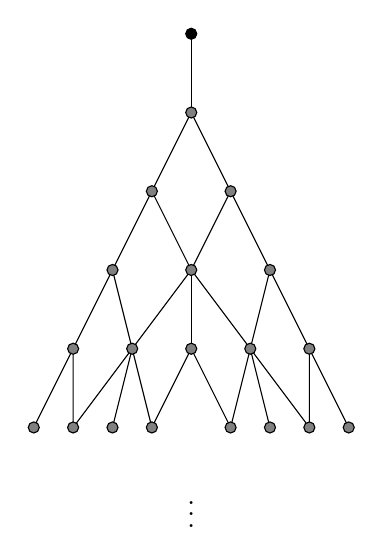
\begin{tikzpicture}[nodes={circle, draw, fill=black!50, inner sep=0pt, minimum width=4pt}]
              \draw (2,-4) -- (1.5,-3) -- (1,-2) -- (0.5,-1) -- (0,0) -- (-0.5,-1) -- (-1,-2) -- (-1.5,-3) -- (-2,-4);
        \draw (1.5,-3) -- (1.5,-4) -- (0.75,-3) -- (0,-2) -- (-0.75,-3) -- (-1.5,-4) -- (-1.5,-3);
        \draw  (1,-4) -- (0.75,-3) -- (0.5,-4) -- (0,-3) -- (-0.5,-4) -- (-0.75,-3) -- (-1,-4);
        \draw (0,-3) -- (0,-2);
        \draw (0.5,-1) -- (0,-2) -- (-0.5,-1);
        \draw (-0.75,-3) -- (-1,-2);
        \draw (0.75,-3) -- (1,-2);
        \draw (0,1) -- (0,0);
        \node[fill=black] at (0,1) {};
        \node at (0,0) {};
        \node at (-0.5,-1) {};
        \node at (0.5,-1) {};
        \node at (0,-2) {};
        \node at (1,-2) {};
        \node at (-1,-2) {};
        \node at (0,-3) {};
        \node at (0.75,-3) {};
        \node at (-0.75,-3) {};
        \node at (1.5,-3) {};
        \node at (-1.5,-3) {};
        \node at (-2,-4) {};
        \node at (-1.5,-4) {};
        \node at (-1,-4) {};
        \node at (-0.5,-4) {};
        \node at (0.5,-4) {};
        \node at (1,-4) {};
        \node at (1.5,-4) {};
        \node at (2,-4) {};
        \node[draw=none, fill=white] at (0,-5) {$\vdots$};
      \end{tikzpicture}
    \end{center}

with the root corresponding to the upper vertex of the square. 

\begin{prop}\label{grad}
Let $\mathfrak{t}$ be a bounded t-structure on $\mathscr{D}$, $\mathscr{P}$ an abelian $\mathbb{Z}$-slicing on $\heartsuit_{\mathfrak{t}}$, $\mathscr{Q}$ the associated $\mathbb{Z} \ltimes \hat{\mathbb{Z}}$-slicing on $\mathscr{D}$, $p$ a perversity. We have: 
\begin{enumerate}
\item if $\mathscr{P}$ is a perverse filtration, then $\mathscr{Q}$ satisfies the assumptions of \hyperref[pipp]{\textbf{Proposition \ref*{pipp}}} with respect to the map $\mathbb{Z} \ltimes \hat{\mathbb{Z}} \overset{f_p}{\longrightarrow} \mathbb{Z} \ltimes \hat{\mathbb{Z}}$ given by $$f_p(n,\phi)=(n+p(\lfloor \phi / 2 \rfloor),-p(\lfloor \phi / 2 \rfloor))$$ 
\item if $\mathscr{P}$ is a grading filtration, then $\mathscr{Q}$ satisfies the assumptions of \hyperref[pipp]{\textbf{Proposition \ref*{pipp}}} with respect to the map $\mathbb{Z} \ltimes \hat{\mathbb{Z}} \overset{g_p}{\longrightarrow} \mathbb{Z} \ltimes \hat{\mathbb{Z}}$ given by $$g_p(n,\phi)=(n+p(\phi),-p(\phi))$$ 
\item if $\mathscr{P}$ is a mixed filtration, then the abelian $\mathbb{Z}$-slicing induced on the heart of the bounded t-structure associated to $(g_p)_{\textnormal{\Libra}}(\mathscr{Q})$ is split 
\end{enumerate}
\end{prop}

\begin{proof}
Let's prove \textit{(2)}. Suppose $g_p(n,\phi) > g_p(m,\psi)$. Then either $m-n< p(\phi) - p(\psi)$ or both $m-n = p(\phi) - p(\psi)$ and $p(\psi) < p(\psi)$. Since by definition of t-structure we can assume $m \ge n$, the second case is absurd while in the first case, since $p$ is monotone, we have $\phi \ge \psi$ and thus by definition of perversity $$m-n<p(\phi)-p(\psi) \le \phi - \psi$$ 
and we get the desired Hom-vanishing by definition of grading filtration. \\

Suppose now $f_p(n,\phi) + 1 > f_p(m,\psi)$ and $(n+1,\phi) < (m,\psi)$. The only non absurd case is $ 1<m-n \le  p(\phi) - p(\psi)$. But then again we have $$2 \le m-n \le p(\phi)-p(\psi) \le \phi - \psi$$
and we can conclude as above. \\

To prove \textit{(1)} consider the monotone map $$\mathbb{Z} \overset{\lfloor * / 2 \rfloor}{\longrightarrow} \mathbb{Z}$$
Applying the slice functor to the latter and starting with a perverse filtration, we get a grading filtration by the properties of the floor function and the thesis follows from part \textit{(2)}. \\ 

Let's prove \textit{(3)}. We have to show that $$\mathscr{P}_{\psi}[1-p(\psi)] \subseteq \mathscr{P}_{\phi }[p(\phi)]^{\perp}$$ 
for $-p(\psi)>-p(\phi)$. We denote $n=p(\phi)-p(\psi)-1$. Assuming again $n \ge 0$, we have $n \ge 0 > p(\psi) - p(\phi) \ge \psi - \phi$ and we can then conclude by definition of mixed filtration. 
\end{proof}

Thus, in the presence of a grading (or perverse) filtration on the heart of a bounded t-structure, associating to a perversity $p$ the bounded t-structure coming from $(g_p)_{\textnormal{\Libra}}(\mathscr{Q})$ defines a morphism of $\mathbb{Z}$-posets $$\Xi^{\textnormal{op}} \longrightarrow \mathfrak{bts}(\mathscr{D})$$
we can restate this as: 

\begin{center}
\twonotes \ \textit{A grading or perverse filtration on the heart of a bounded t-structure on $\mathscr{D}$ induces a presheaf of t-structures on $\mathbb{Z} \times \mathbb{Z}$ with the product order, and thus some kind of a 'non totally ordered $\mathbb{Z} \times \mathbb{Z}$-slicing' on $\mathscr{D}$.}
\end{center}

\begin{center}
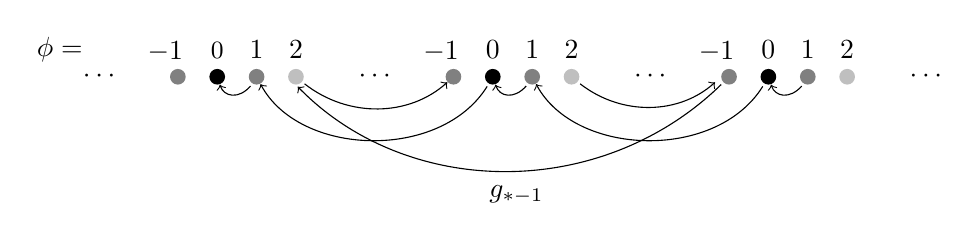
\begin{tikzpicture}

\node at (-5,0) {$\cdots$};
\draw (-4,0) node[circle,fill=gray,inner sep=2pt,label={[xshift=-4.5pt, yshift=-1pt]above: $-1$}] {};
\draw (-3.5,0) node[circle,fill,inner sep=2pt,label={[font=\small]above: $0$}] {};
\draw (-3,0) node[circle,fill=gray,inner sep=2pt,label=above: {$1$}] {} edge[->, bend left=60,looseness=1.5,shorten <=1pt,shorten >=3pt] (-3.5,0);
\draw (-2.5,0) node[circle,fill=lightgray,inner sep=2pt,label=above: {$2$}] {} edge[->, bend right=40,shorten <=1pt,shorten >=3pt] (-0.5,0);

\node at (-1.5,0) {$\cdots$};
\draw (-0.5,0) node[circle,fill=gray,inner sep=2pt,label={[xshift=-4.5pt, yshift=-1pt]above: $-1$}] {};
\draw (0,0) node[circle,fill,inner sep=2pt,label=above: {$0$}] {}  edge[->, bend left=60,shorten <=1pt,shorten >=3pt] (-3,0);
\draw (0.5,0) node[circle,fill=gray,inner sep=2pt,label=above: {$1$}] {} edge[->, bend left=60,looseness=1.5,shorten <=1pt,shorten >=3pt] (0,0);
\draw (1,0) node[circle,fill=lightgray,inner sep=2pt,label=above: {$2$}] {}  edge[->, bend right=40,shorten <=1pt,shorten >=3pt] (2.9,0);
\node at (2,0) {$\cdots$};

\draw (3,0) node[circle,fill=gray,inner sep=2pt,label={[xshift=-4.5pt, yshift=-1pt]above: $-1$}] {} edge[->, bend left=45,shorten <=1pt,shorten >=5pt] (-2.6,0);
\draw (3.5,0) node[circle,fill,inner sep=2pt,label=above: {$0$}] {} edge[->, bend left=60,shorten <=1pt,shorten >=3pt] (0.5,0);
\draw (4,0) node[circle,fill=gray,inner sep=2pt,label=above: {$1$}] {} edge[->, bend left=60,looseness=1.5,shorten <=1pt,shorten >=3pt] (3.5,0);
\draw (4.5,0) node[circle,fill=lightgray,inner sep=2pt,label=above: {$2$}] {};
\node at (5.5,0) {$\cdots$};

\node at (-5.5,0.35) {$\phi=$};
\node at (0.3,-1.5) {$g_{*-1}$};

\end{tikzpicture}
\end{center}

Now, by sending an upper set of $I \in O(\mathbb{Z})$ to its characteristic function $\chi_I$ we get an embedding $$O(\mathbb{Z})^{\textnormal{op}} \hookrightarrow \Xi$$ and the t-structure coming from $(g_{\chi_I})_{\textnormal{\Libra}}(\mathscr{Q})$ is just the tilting of $\mathfrak{t}$ with respect to the torsion pair coming from $I$. \\
The following proposition gives a characterization of the new heart obtained by the above construction. In the case of a mixed filtration, we get a splitting property which is often referred as 'decomposition theorem for perverse sheaves' in literature. \\

\begin{prop}
Let $\mathfrak{t}$ be a bounded t-structure on $\mathscr{D}$, $\mathscr{P}$ a grading filtration on $\heartsuit_{\mathfrak{t}}$, $\mathscr{Q}$ the associated $\mathbb{Z} \ltimes \hat{\mathbb{Z}}$-slicing on $\mathscr{D}$, $p$ a perversity. Denote $\mathfrak{q}$ the bounded t-structure associated to $(g_p)_{\textnormal{\Libra}}(\mathscr{Q})$. Then $\heartsuit_{\mathfrak{q}}$ consists of objects $X \in \mathscr{D}$ so that $$H_{\mathfrak{t}}^{k}(X) \in \mathscr{P}_{p^{-1}(-k)}[k]$$ 
for each $k \in \mathbb{Z}$. Moreover, if $\mathscr{P}$ is a mixed filtration then for each $X \in \heartsuit_{\mathfrak{q}}$ $$X=\bigoplus_{n \in \mathbb{Z}}H_{\mathfrak{t}}^{n}(X)$$ 
\end{prop}

\begin{proof}
This is very similar to \hyperref[tilt1]{\textbf{Proposition \ref*{tilt1}}}: we have that $X \in \heartsuit_{\mathfrak{q}}$ if and only if $$H_{\mathscr{P}}^{\phi}(H_{\mathfrak{t}}^k(X)[-k])[k]=H_{\mathscr{Q}}^{(k,\phi)}(X)=0$$ 
for $p(\phi) \not = -k$. \\
For the second part of the claim, the abelian $\mathbb{Z}$-slicing induced on $\heartsuit_{\mathfrak{q}}$ is split by \hyperref[grad]{\textbf{Proposition \ref*{grad}}} and thus by \hyperref[split]{\textbf{Proposition \ref*{split}}} $$X=\bigoplus_{(k,\phi)}H_{\mathscr{Q}}^{(k,\phi)}(X)=\bigoplus_{n \in \mathbb{Z}}H_{\mathfrak{t}}^{n}(X)$$
where the last equality comes from the first part. 
\end{proof}

\begin{exmp}
Let $$B=\bigoplus_{i\in \mathbb{N}}B_i$$ be an $\mathbb{N}$-graded ring with $B_0$ semisimple. Denote $\mathscr{A}$ the category of $\mathbb{Z}$-graded $B$-modules with only finitely many nonzero graded pieces. For $\phi \in \mathbb{Z}$, denote $\mathscr{P}_{\phi}$ the full subcategory of $\mathscr{A}$ of modules concentrated in degree $\phi$. Clearly, $\mathscr{P}$ defines an abelian $\mathbb{Z}$-slicing on $\mathscr{A}$. Following \cite{kos} we have $$\textnormal{Ext}_{\mathscr{A}}^n(\mathscr{P}_{\phi},\mathscr{P}_{\psi})=0$$
for $n>\psi - \phi$. This means that $\mathscr{P}$ is a mixed filtration and the bounded t-structure on $\mathscr{D}^b(\mathscr{A})$ associated to $(g_1)_{\textnormal{\Libra}}(\mathscr{Q})$ (where $1$ is the identity of $\mathbb{Z}$) is the 'diagonal' (or 'geometric') t-structure which appears in Koszul duality and other areas. 
\end{exmp}

\begin{exmp}
Let $M$ be an $n$-dimensional smooth complex projective variety and consider the $n$-torsion pair $\mathscr{P}$ on $\textnormal{Coh}(M)$ from \hyperref[cohh]{\textbf{Example \ref*{cohh}}}. Using Serre duality and the Grothendieck vanishing theorem, one sees that $\mathscr{P}$, seen as an abelian $\mathbb{Z}$-slicing via the inclusion $[n] \subseteq \mathbb{Z}$, is a perverse filtration. The bounded t-structure associated to $(f_p)_{\textnormal{\Libra}}(\mathscr{Q})$ is the one of perverse coherent sheaves as constructed in \cite{bez}. Following again the proof of \hyperref[t]{\textbf{Proposition \ref*{t}}}, we can use the Harder-Narasimhan filtrations from Gieseker stability to obtain an abelian $J_n$-slicing on the heart of perverse coherent sheaves as done in \cite{perpol}. 
\end{exmp}

Now we somehow review the gluing construction for t-structures in \cite{del}, but generalize it to any slicing. Our language is quite different though, and we formulate the problem very similarly to \cite{glu}. We start with two $\mathbb{Z}$-posets $J,J'$. 

\begin{defn}
Let $\mathscr{P}$ be a $J \ltimes J'$-slicing on $\mathscr{D}$. We call $\mathscr{P}$ \textbf{gluable} if it satisties the assumptions of \hyperref[pipp]{\textbf{Proposition \ref*{pipp}}} with respect to the map $J \ltimes J' \overset{e}{\longrightarrow} J' \ltimes J$ that exchanges coordinates. In this case we denote $$\overline{\mathscr{P}}=e_{\textnormal{\Libra}}(\mathscr{P})$$
\end{defn}

By a simple computation, the gluability condition reads: $\mathscr{P}_{(\phi,\psi)} \subseteq \mathscr{P}_{(\phi',\psi')}^{\perp}$ if $\psi' > \psi$ or both $\psi'+1>\psi$ and $\phi'+1 < \phi$. For example, the first condition is automatic when $\mathbb{Z}$ acts trivially on $J$ (in this case, it follows from the second one). In particular, if $\mathbb{Z}$ acts trivially on $J$, $\mathscr{P}$ is a $J$-slicing on $\mathscr{D}$ and $\mathfrak{t}_{\phi}$ is a bounded t-structure on $\mathscr{P}_{\phi}$ for each $\phi \in J$, then using \hyperref[aab]{\textbf{Proposition \ref*{aab}}} we get a $J \ltimes \mathbb{Z}$-slicing $\mathscr{Q}$ which is gluable if and only if $$\heartsuit_{\mathfrak{t}_{\psi}}[n] \subseteq \heartsuit_{\mathfrak{t}_{\phi}}^{\perp}$$
whenever both $n \le 0$ and $\phi < \psi$. 

\begin{rem}
We have a commutative diagram of $\mathbb{Z}$-posets 
\begin{center}
\begin{tikzcd}[ampersand replacement=\&]
\mathbb{Z} \ltimes \mathbb{Z} \arrow{r}{\sim} \arrow{d}{e} \& \mathbb{Z} \ltimes \hat{\mathbb{Z}} \arrow{d}{g} \\
\mathbb{Z} \ltimes \mathbb{Z} \arrow{r}{\sim}  \& \mathbb{Z} \ltimes \hat{\mathbb{Z}} 
\end{tikzcd}
\end{center}
where the horizontal isomorphism is the one from \hyperref[zet]{\textbf{Remark \ref*{zet}}}. Indeed, a $\mathbb{Z} \ltimes \mathbb{Z}$-slicing on $\mathscr{D}$ is gluable if and only if it induces a grading filtration on the heart of the associated t-structure when seen as a $\mathbb{Z} \ltimes \hat{\mathbb{Z}}$-slicing. 
\end{rem} 

An easy combinatorial calculation finally yelds the following two remarks: 
\begin{itemize}
\item  if $\mathscr{P}$ is a gluable $\hat{\mathbb{Z}} \ltimes \mathbb{Z}$-slicing on $\mathscr{D}$, then $\overline{\mathscr{P}}$ induces a grading filtration on the associated heart, allowing us again to construct new bounded t-structures depending on a perversity. 
\item if $\mathscr{P}$ is a mixed filtration on the heart of a bounded t-structure and $\mathscr{Q}$ is the associated $\mathbb{Z} \ltimes \hat{\mathbb{Z}}$-slicing on $\mathscr{D}$, then $\mathscr{Q}$ is gluable. In this case, looking at $\overline{\mathscr{Q}}$, we get a baric structure on $\mathscr{D}$ which is usually called \textbf{weight decomposition} in literature. 
\end{itemize}
In other words, the chain of implications for a $\mathbb{Z} \ltimes \hat{\mathbb{Z}}$-slicing refines to 
$$\textnormal{mixed} \implies \textnormal{gluable} \implies \textnormal{grading} \implies \textnormal{perverse} $$

%\begin{prop}
%A $J \ltimes J'$-slicing $\mathscr{P}$ on $\mathscr{D}$ is gluable if and only if it satifies the assumptions of \hyperref[pipp]{\textbf{Proposition \ref*{pipp}}} with respect to the identity (as sets) $J \ltimes J' \longrightarrow J \times J'$, where we place the product order on the right member. 
%\end{prop}
%
%\begin{proof}
 % Consider the following commutative diagram of sets
 % \begin{center}
%\begin{tikzcd}[ampersand replacement=\&]
%J \ltimes J' \arrow{r}{e} \arrow{d}{1} \& J \ltimes J' \\
%J \times J' \arrow{r}{e}  \& J \times J' \arrow{u}{1}
%\end{tikzcd}
%  \end{center}
%  The right arrow is a morphism of $\mathbb{Z}$-posets while the down one is an isomorphism of $\mathbb{Z}$-posets, and the thesis follows. 
%\end{proof}
%\begin{prop}
%Let $\mathscr{P}$ be a gluable $J \times J'$-slicing on $\mathscr{D}$. For $i = 1,2$, denote $\mathscr{P}^i=\pi_{\textnormal{\Libra}}^i(\mathscr{P})$, where $J \overset{\pi^1}{\longleftarrow} J \times J' \overset{\pi^2}{\longrightarrow} J'$ are the projections. Then for each $\psi \in J'$, $\mathscr{P}_{\psi}^2$ consists of objects $X \in \mathscr{D}$ so that $$H_{\mathscr{P}^1}^{\phi}(X) \in \mathscr{Q}_{(\phi,\psi)}$$
%for each $\phi \in J$.
%\end{prop}
%
%\begin{proof}
%We have already seen that $X \in \mathscr{P}_{\psi}^2$ if and only if $$H_{\mathscr{P}}^{\lambda}(X)=H_{\mathscr{P}}^{\lambda}(H_{\mathscr{P}^1}^{\pi^1(\lambda)}(X))=0$$
%for $\pi^2(\lambda) \not =\psi$. By fixing $\pi^1(\lambda)=\phi$ and varying $\pi^2(\lambda)$, we get the desired result. 
%\end{proof}
\newpage
